\documentclass[preprint,12pt]{elsarticle}
% IP&M (Information Processing & Management) submission.
% Switch to [review,12pt] to add line numbers for referees.

\usepackage[T1]{fontenc}
\usepackage{amsmath, amsfonts}
\usepackage{amssymb}
\usepackage{mathtools}
\usepackage{graphicx}
\usepackage{booktabs}
\usepackage{microtype}
\usepackage{xcolor}
\usepackage{xurl}
\usepackage[ruled]{algorithm2e}
\usepackage[inline, shortlabels]{enumitem}
\usepackage{hyperref}
\usepackage{caption}
\DeclarePairedDelimiterX\p[1]{(}{)}{#1}
\DeclarePairedDelimiter\Bset{[}{]}
\DeclarePairedDelimiter\abs{\lvert}{\rvert}
\usepackage{amsthm}
\newtheorem{proposition}{Proposition}
\newtheorem{condition}{Condition}
\theoremstyle{remark}

% Auto-generated by scripts/make_numbers_journal.py. Do not edit.
% ---- Table 2: evidence recall at r=4, three datasets ----
\newcommand{\RecQSie}{36.2}
\newcommand{\RecQSieLo}{33.9}
\newcommand{\RecQSieHi}{38.5}
\newcommand{\RecQBm}{43.1}
\newcommand{\RecQBmLo}{41.0}
\newcommand{\RecQBmHi}{45.2}
\newcommand{\RecQHea}{23.4}
\newcommand{\RecQHeaLo}{20.8}
\newcommand{\RecQHeaHi}{26.0}
\newcommand{\RecQRan}{26.0}
\newcommand{\RecQRanLo}{24.5}
\newcommand{\RecQRanHi}{27.4}
\newcommand{\RecQStr}{22.2}
\newcommand{\RecQStrLo}{21.2}
\newcommand{\RecQStrHi}{23.2}
\newcommand{\RecQTR}{26.3}
\newcommand{\RecQTRLo}{24.7}
\newcommand{\RecQTRHi}{28.1}
\newcommand{\RecHSie}{66.7}
\newcommand{\RecHSieLo}{63.2}
\newcommand{\RecHSieHi}{69.8}
\newcommand{\RecHBm}{73.1}
\newcommand{\RecHBmLo}{69.8}
\newcommand{\RecHBmHi}{76.2}
\newcommand{\RecHHea}{22.0}
\newcommand{\RecHHeaLo}{19.0}
\newcommand{\RecHHeaHi}{25.0}
\newcommand{\RecHRan}{27.4}
\newcommand{\RecHRanLo}{24.1}
\newcommand{\RecHRanHi}{30.7}
\newcommand{\RecHStr}{26.6}
\newcommand{\RecHStrLo}{23.4}
\newcommand{\RecHStrHi}{29.7}
\newcommand{\RecHTR}{35.6}
\newcommand{\RecHTRLo}{32.5}
\newcommand{\RecHTRHi}{39.1}
\newcommand{\RecWSie}{50.5}
\newcommand{\RecWSieLo}{46.8}
\newcommand{\RecWSieHi}{54.3}
\newcommand{\RecWBm}{57.6}
\newcommand{\RecWBmLo}{53.6}
\newcommand{\RecWBmHi}{61.5}
\newcommand{\RecWHea}{27.7}
\newcommand{\RecWHeaLo}{24.3}
\newcommand{\RecWHeaHi}{30.8}
\newcommand{\RecWRan}{25.9}
\newcommand{\RecWRanLo}{22.6}
\newcommand{\RecWRanHi}{29.2}
\newcommand{\RecWStr}{21.4}
\newcommand{\RecWStrLo}{18.4}
\newcommand{\RecWStrHi}{24.4}
\newcommand{\RecWTR}{38.1}
\newcommand{\RecWTRLo}{34.2}
\newcommand{\RecWTRHi}{41.8}
\newcommand{\NRecQ}{1000}
\newcommand{\NRecH}{300}
\newcommand{\NRecW}{300}
% ---- paired intervals (recall points) ----
\newcommand{\PairQSH}{12.8}
\newcommand{\PairQSHLo}{10.0}
\newcommand{\PairQSHHi}{15.3}
\newcommand{\PairQSBm}{-6.8}
\newcommand{\PairQSBmLo}{-8.7}
\newcommand{\PairQSBmHi}{-5.0}
\newcommand{\PairQSTR}{9.9}
\newcommand{\PairQSTRLo}{7.2}
\newcommand{\PairQSTRHi}{12.8}
\newcommand{\PairHSH}{44.8}
\newcommand{\PairHSHLo}{40.7}
\newcommand{\PairHSHHi}{48.9}
\newcommand{\PairHSBm}{-6.3}
\newcommand{\PairHSBmLo}{-9.0}
\newcommand{\PairHSBmHi}{-3.7}
\newcommand{\PairHSTR}{31.1}
\newcommand{\PairHSTRLo}{26.3}
\newcommand{\PairHSTRHi}{35.3}
\newcommand{\PairWSH}{22.8}
\newcommand{\PairWSHLo}{18.2}
\newcommand{\PairWSHHi}{27.2}
\newcommand{\PairWSBm}{-7.1}
\newcommand{\PairWSBmLo}{-10.5}
\newcommand{\PairWSBmHi}{-4.0}
\newcommand{\PairWSTR}{12.4}
\newcommand{\PairWSTRLo}{7.2}
\newcommand{\PairWSTRHi}{17.9}
% ---- ratio sweep (values used in text; figure reads JSON) ----
\newcommand{\RatQSieTwo}{57.9}
\newcommand{\RatQSieTwoLo}{55.4}
\newcommand{\RatQSieTwoHi}{60.2}
\newcommand{\RatQBmTwo}{61.1}
\newcommand{\RatQBmTwoLo}{58.8}
\newcommand{\RatQBmTwoHi}{63.4}
\newcommand{\RatQHeaTwo}{50.0}
\newcommand{\RatQHeaTwoLo}{46.7}
\newcommand{\RatQHeaTwoHi}{53.1}
\newcommand{\RatQRanTwo}{50.1}
\newcommand{\RatQRanTwoLo}{48.4}
\newcommand{\RatQRanTwoHi}{51.7}
\newcommand{\RatQTRTwo}{51.3}
\newcommand{\RatQTRTwoLo}{49.3}
\newcommand{\RatQTRTwoHi}{53.1}
\newcommand{\RatQSieFour}{36.2}
\newcommand{\RatQSieFourLo}{33.9}
\newcommand{\RatQSieFourHi}{38.5}
\newcommand{\RatQBmFour}{43.1}
\newcommand{\RatQBmFourLo}{41.0}
\newcommand{\RatQBmFourHi}{45.2}
\newcommand{\RatQHeaFour}{23.4}
\newcommand{\RatQHeaFourLo}{20.8}
\newcommand{\RatQHeaFourHi}{26.0}
\newcommand{\RatQRanFour}{26.0}
\newcommand{\RatQRanFourLo}{24.5}
\newcommand{\RatQRanFourHi}{27.4}
\newcommand{\RatQTRFour}{26.3}
\newcommand{\RatQTRFourLo}{24.7}
\newcommand{\RatQTRFourHi}{28.1}
\newcommand{\RatQSieEight}{23.9}
\newcommand{\RatQSieEightLo}{22.0}
\newcommand{\RatQSieEightHi}{25.8}
\newcommand{\RatQBmEight}{31.0}
\newcommand{\RatQBmEightLo}{29.0}
\newcommand{\RatQBmEightHi}{32.8}
\newcommand{\RatQHeaEight}{10.6}
\newcommand{\RatQHeaEightLo}{8.8}
\newcommand{\RatQHeaEightHi}{12.5}
\newcommand{\RatQRanEight}{13.4}
\newcommand{\RatQRanEightLo}{12.3}
\newcommand{\RatQRanEightHi}{14.5}
\newcommand{\RatQTREight}{14.0}
\newcommand{\RatQTREightLo}{12.8}
\newcommand{\RatQTREightHi}{15.4}
\newcommand{\RatQSieSixteen}{15.6}
\newcommand{\RatQSieSixteenLo}{14.2}
\newcommand{\RatQSieSixteenHi}{17.1}
\newcommand{\RatQBmSixteen}{21.5}
\newcommand{\RatQBmSixteenLo}{19.9}
\newcommand{\RatQBmSixteenHi}{23.1}
\newcommand{\RatQHeaSixteen}{4.4}
\newcommand{\RatQHeaSixteenLo}{3.3}
\newcommand{\RatQHeaSixteenHi}{5.7}
\newcommand{\RatQRanSixteen}{6.6}
\newcommand{\RatQRanSixteenLo}{5.7}
\newcommand{\RatQRanSixteenHi}{7.5}
\newcommand{\RatQTRSixteen}{7.5}
\newcommand{\RatQTRSixteenLo}{6.6}
\newcommand{\RatQTRSixteenHi}{8.5}
\newcommand{\RatHSieTwo}{84.1}
\newcommand{\RatHSieTwoLo}{81.5}
\newcommand{\RatHSieTwoHi}{86.7}
\newcommand{\RatHBmTwo}{86.7}
\newcommand{\RatHBmTwoLo}{84.1}
\newcommand{\RatHBmTwoHi}{89.0}
\newcommand{\RatHHeaTwo}{44.1}
\newcommand{\RatHHeaTwoLo}{39.9}
\newcommand{\RatHHeaTwoHi}{48.1}
\newcommand{\RatHRanTwo}{53.5}
\newcommand{\RatHRanTwoLo}{50.0}
\newcommand{\RatHRanTwoHi}{57.2}
\newcommand{\RatHTRTwo}{62.3}
\newcommand{\RatHTRTwoLo}{58.9}
\newcommand{\RatHTRTwoHi}{65.7}
\newcommand{\RatHSieFour}{66.7}
\newcommand{\RatHSieFourLo}{63.2}
\newcommand{\RatHSieFourHi}{69.8}
\newcommand{\RatHBmFour}{73.1}
\newcommand{\RatHBmFourLo}{69.8}
\newcommand{\RatHBmFourHi}{76.2}
\newcommand{\RatHHeaFour}{22.0}
\newcommand{\RatHHeaFourLo}{19.0}
\newcommand{\RatHHeaFourHi}{25.0}
\newcommand{\RatHRanFour}{27.4}
\newcommand{\RatHRanFourLo}{24.1}
\newcommand{\RatHRanFourHi}{30.7}
\newcommand{\RatHTRFour}{35.6}
\newcommand{\RatHTRFourLo}{32.5}
\newcommand{\RatHTRFourHi}{39.1}
\newcommand{\RatHSieEight}{52.2}
\newcommand{\RatHSieEightLo}{48.4}
\newcommand{\RatHSieEightHi}{55.7}
\newcommand{\RatHBmEight}{60.0}
\newcommand{\RatHBmEightLo}{56.7}
\newcommand{\RatHBmEightHi}{63.2}
\newcommand{\RatHHeaEight}{13.0}
\newcommand{\RatHHeaEightLo}{10.5}
\newcommand{\RatHHeaEightHi}{15.6}
\newcommand{\RatHRanEight}{12.1}
\newcommand{\RatHRanEightLo}{9.9}
\newcommand{\RatHRanEightHi}{14.5}
\newcommand{\RatHTREight}{20.2}
\newcommand{\RatHTREightLo}{17.3}
\newcommand{\RatHTREightHi}{23.2}
\newcommand{\RatHSieSixteen}{38.6}
\newcommand{\RatHSieSixteenLo}{35.3}
\newcommand{\RatHSieSixteenHi}{41.7}
\newcommand{\RatHBmSixteen}{44.9}
\newcommand{\RatHBmSixteenLo}{41.7}
\newcommand{\RatHBmSixteenHi}{48.2}
\newcommand{\RatHHeaSixteen}{7.6}
\newcommand{\RatHHeaSixteenLo}{5.8}
\newcommand{\RatHHeaSixteenHi}{9.5}
\newcommand{\RatHRanSixteen}{5.3}
\newcommand{\RatHRanSixteenLo}{3.8}
\newcommand{\RatHRanSixteenHi}{7.1}
\newcommand{\RatHTRSixteen}{12.0}
\newcommand{\RatHTRSixteenLo}{9.7}
\newcommand{\RatHTRSixteenHi}{14.3}
\newcommand{\RatWSieTwo}{72.9}
\newcommand{\RatWSieTwoLo}{69.4}
\newcommand{\RatWSieTwoHi}{76.4}
\newcommand{\RatWBmTwo}{75.0}
\newcommand{\RatWBmTwoLo}{71.7}
\newcommand{\RatWBmTwoHi}{78.5}
\newcommand{\RatWHeaTwo}{53.2}
\newcommand{\RatWHeaTwoLo}{49.6}
\newcommand{\RatWHeaTwoHi}{56.8}
\newcommand{\RatWRanTwo}{52.8}
\newcommand{\RatWRanTwoLo}{49.0}
\newcommand{\RatWRanTwoHi}{56.8}
\newcommand{\RatWTRTwo}{63.2}
\newcommand{\RatWTRTwoLo}{58.9}
\newcommand{\RatWTRTwoHi}{67.3}
\newcommand{\RatWSieFour}{50.5}
\newcommand{\RatWSieFourLo}{46.8}
\newcommand{\RatWSieFourHi}{54.3}
\newcommand{\RatWBmFour}{57.6}
\newcommand{\RatWBmFourLo}{53.6}
\newcommand{\RatWBmFourHi}{61.5}
\newcommand{\RatWHeaFour}{27.7}
\newcommand{\RatWHeaFourLo}{24.3}
\newcommand{\RatWHeaFourHi}{30.8}
\newcommand{\RatWRanFour}{25.9}
\newcommand{\RatWRanFourLo}{22.6}
\newcommand{\RatWRanFourHi}{29.2}
\newcommand{\RatWTRFour}{38.1}
\newcommand{\RatWTRFourLo}{34.2}
\newcommand{\RatWTRFourHi}{41.8}
\newcommand{\RatWSieEight}{35.2}
\newcommand{\RatWSieEightLo}{31.8}
\newcommand{\RatWSieEightHi}{38.5}
\newcommand{\RatWBmEight}{41.7}
\newcommand{\RatWBmEightLo}{38.0}
\newcommand{\RatWBmEightHi}{45.3}
\newcommand{\RatWHeaEight}{14.7}
\newcommand{\RatWHeaEightLo}{12.0}
\newcommand{\RatWHeaEightHi}{17.4}
\newcommand{\RatWRanEight}{12.2}
\newcommand{\RatWRanEightLo}{9.7}
\newcommand{\RatWRanEightHi}{14.7}
\newcommand{\RatWTREight}{20.7}
\newcommand{\RatWTREightLo}{17.4}
\newcommand{\RatWTREightHi}{23.7}
\newcommand{\RatWSieSixteen}{24.5}
\newcommand{\RatWSieSixteenLo}{21.6}
\newcommand{\RatWSieSixteenHi}{27.4}
\newcommand{\RatWBmSixteen}{30.0}
\newcommand{\RatWBmSixteenLo}{26.8}
\newcommand{\RatWBmSixteenHi}{33.3}
\newcommand{\RatWHeaSixteen}{8.6}
\newcommand{\RatWHeaSixteenLo}{6.5}
\newcommand{\RatWHeaSixteenHi}{10.8}
\newcommand{\RatWRanSixteen}{5.8}
\newcommand{\RatWRanSixteenLo}{4.1}
\newcommand{\RatWRanSixteenHi}{7.8}
\newcommand{\RatWTRSixteen}{12.1}
\newcommand{\RatWTRSixteenLo}{9.6}
\newcommand{\RatWTRSixteenHi}{14.5}
% ---- selector ablations (QASPER) ----
\newcommand{\AblSie}{36.2}
\newcommand{\AblNoQ}{19.9}
\newcommand{\AblNoPos}{43.3}
\newcommand{\AblNoRed}{36.3}
\newcommand{\AblRelOnly}{43.6}
% ---- position study ----
\newcommand{\PosStart}{97.7}
\newcommand{\PosStartN}{1000}
\newcommand{\PosQuarter}{37.0}
\newcommand{\PosQuarterN}{1000}
\newcommand{\PosHalf}{21.9}
\newcommand{\PosHalfN}{1000}
\newcommand{\PosThreeQ}{36.7}
\newcommand{\PosThreeQN}{1000}
\newcommand{\PosEnd}{97.3}
\newcommand{\PosEndN}{1000}
% ---- sensitivity ----
\newcommand{\SensBetaZp}{36.3}
\newcommand{\SensBetaMid}{36.2}
\newcommand{\SensBetaHigh}{36.3}
\newcommand{\SensFloorZp}{32.1}
\newcommand{\SensFloorMid}{36.2}
\newcommand{\SensFloorHigh}{41.2}
\newcommand{\SensFloorOne}{43.3}
\newcommand{\SensGammaLo}{39.0}
\newcommand{\SensGammaMid}{36.2}
\newcommand{\SensGammaHigh}{36.9}
% ---- pool statistics ----
\newcommand{\PoolQN}{1000}
\newcommand{\PoolQMedPos}{48}
\newcommand{\PoolQEvSents}{4.8}
\newcommand{\PoolQMedWords}{3538}
\newcommand{\PoolHN}{300}
\newcommand{\PoolHMedPos}{54}
\newcommand{\PoolHEvSents}{2.5}
\newcommand{\PoolHMedWords}{888}
\newcommand{\PoolWN}{300}
\newcommand{\PoolWMedPos}{46}
\newcommand{\PoolWEvSents}{2.4}
\newcommand{\PoolWMedWords}{602}
\newcommand{\TotalRecords}{1600}
% ---- GPT-2 perplexity gate ----
\newcommand{\GateRecall}{28.7}
\newcommand{\GateRecallLo}{20.4}
\newcommand{\GateRecallHi}{37.7}
\newcommand{\GateN}{100}
\newcommand{\GateLatMedS}{7.5}
\newcommand{\GateLatMedCtxS}{8.2}
\newcommand{\GateLatPnineS}{13.1}
\newcommand{\GateLatSixkS}{12.7}
\newcommand{\GateSixkN}{17}
\newcommand{\GateMedWords}{3591}
\newcommand{\GateMedTok}{5410}
% ---- timing benchmark (ms, same container) ----
\newcommand{\TimeSieOnek}{3.3}
\newcommand{\TimeTROnek}{6.4}
\newcommand{\TimeHeaOnek}{0.1}
\newcommand{\TimeRanOnek}{1.2}
\newcommand{\TimeStrOnek}{1.2}
\newcommand{\TimeBmOnek}{1.8}
\newcommand{\TimeSieTwok}{9.0}
\newcommand{\TimeTRTwok}{20.0}
\newcommand{\TimeHeaTwok}{0.1}
\newcommand{\TimeRanTwok}{2.5}
\newcommand{\TimeStrTwok}{2.5}
\newcommand{\TimeBmTwok}{3.6}
\newcommand{\TimeSieFourk}{29.9}
\newcommand{\TimeTRFourk}{69.2}
\newcommand{\TimeHeaFourk}{0.2}
\newcommand{\TimeRanFourk}{5.0}
\newcommand{\TimeStrFourk}{5.1}
\newcommand{\TimeBmFourk}{7.0}
\newcommand{\TimeSieSixk}{53.7}
\newcommand{\TimeTRSixk}{126.0}
\newcommand{\TimeHeaSixk}{0.3}
\newcommand{\TimeRanSixk}{7.5}
\newcommand{\TimeStrSixk}{7.6}
\newcommand{\TimeBmSixk}{10.6}
\newcommand{\TimeGateOnek}{2307.8}
\newcommand{\TimeGateTwok}{4910.1}
\newcommand{\TimeGateFourk}{9288.8}
\newcommand{\TimeGateSixk}{13678.2}
\newcommand{\GateSieRatioSixk}{255}
\newcommand{\GateSieRatioMed}{320}
\newcommand{\GateAOneFloorMs}{10.8}
\newcommand{\BmSpeedup}{5}
% ---- end-task QA (conference protocol: QASPER n=25) ----
\newcommand{\QAFullEM}{20.0}
\newcommand{\QAFullF}{32.1}
\newcommand{\QAFullFlo}{16.2}
\newcommand{\QAFullFhi}{49.5}
\newcommand{\QAFullN}{25}
\newcommand{\QAFullTok}{4993}
\newcommand{\QAHeaEM}{8.0}
\newcommand{\QAHeaF}{20.7}
\newcommand{\QAHeaFlo}{9.5}
\newcommand{\QAHeaFhi}{33.7}
\newcommand{\QAHeaN}{25}
\newcommand{\QAHeaTok}{1248}
\newcommand{\QAHeaDelta}{11.4}
\newcommand{\QAHeaRetain}{64.4}
\newcommand{\QARanEM}{8.0}
\newcommand{\QARanF}{14.3}
\newcommand{\QARanFlo}{4.2}
\newcommand{\QARanFhi}{26.4}
\newcommand{\QARanN}{25}
\newcommand{\QARanTok}{1283}
\newcommand{\QARanDelta}{17.9}
\newcommand{\QARanRetain}{44.4}
\newcommand{\QAStrEM}{4.2}
\newcommand{\QAStrF}{15.0}
\newcommand{\QAStrFlo}{4.8}
\newcommand{\QAStrFhi}{28.1}
\newcommand{\QAStrN}{24}
\newcommand{\QAStrTok}{1140}
\newcommand{\QAStrDelta}{17.1}
\newcommand{\QAStrRetain}{46.7}
\newcommand{\QATREM}{4.2}
\newcommand{\QATRF}{15.5}
\newcommand{\QATRFlo}{4.9}
\newcommand{\QATRFhi}{28.4}
\newcommand{\QATRN}{24}
\newcommand{\QATRTok}{1323}
\newcommand{\QATRDelta}{16.6}
\newcommand{\QATRRetain}{48.4}
\newcommand{\QASieEM}{8.0}
\newcommand{\QASieF}{18.6}
\newcommand{\QASieFlo}{7.6}
\newcommand{\QASieFhi}{31.0}
\newcommand{\QASieN}{25}
\newcommand{\QASieTok}{1249}
\newcommand{\QASieDelta}{13.5}
\newcommand{\QASieRetain}{57.9}
\newcommand{\QAPairSH}{-2.1}
\newcommand{\QAPairSHLo}{-14.5}
\newcommand{\QAPairSHHi}{8.2}
\newcommand{\QAPairSRan}{4.3}
\newcommand{\QAPairSRanLo}{-9.6}
\newcommand{\QAPairSRanHi}{17.6}
\newcommand{\QAPairSTR}{3.8}
\newcommand{\QAPairSTRLo}{-5.4}
\newcommand{\QAPairSTRHi}{12.7}
\newcommand{\QAProto}{conference}
\newcommand{\QAN}{25}
\newcommand{\GridALo}{52.6}
\newcommand{\GridAMid}{47.1}
\newcommand{\GridAHi}{50.4}
\newcommand{\QAReaderMs}{731}
\newcommand{\TotalCalls}{256}
% ---- recall <-> F1 correlation ----
\newcommand{\CorrProto}{conference}
\newcommand{\CorrPearson}{0.30}
\newcommand{\CorrSpearman}{0.30}
\newcommand{\CorrNPairs}{108}
\newcommand{\CorrNRecs}{22}
\newcommand{\CorrSiePearson}{0.34}
\newcommand{\CorrSieSpearman}{0.47}
\newcommand{\CorrHeaPearson}{0.16}
\newcommand{\CorrHeaSpearman}{0.20}
\newcommand{\CorrTRPearson}{0.53}
\newcommand{\CorrTRSpearman}{0.37}


% --- end-task QA protocol helpers -------------------------------
% The expanded end-task protocol (n=100 incl. BM25) defines the \QABm*
% macros; under the conference protocol they are absent and the BM25
% cells fall back to an em dash. \QAProto and \QAN (from numbers.tex)
% record which protocol produced the \QA* macros.
\newcommand{\QAorDash}[2]{%
  \ifcsname QA#1#2\endcsname\csname QA#1#2\endcsname\else--\fi}
\newcommand{\QARetainOrDash}[1]{%
  \ifcsname QA#1Retain\endcsname\csname QA#1Retain\endcsname\%\else--\fi}

\newcommand{\method}{Sieve}
\newcommand{\eg}{e.g.,}
\newcommand{\ie}{i.e.,}
\newcommand{\ms}{\ensuremath{\mathrm{ms}}}

\journal{Information Processing \& Management}

% TODO(author): fill in the real author block before submission.
\author{First Author\corref{cor1}}
\cortext[cor1]{Corresponding author.}
\ead{first.author@example.org}
\address{Affiliation, City, Country}

\begin{document}

\begin{frontmatter}

\title{Sieve: Training-Free, Model-Free, Question-Conditioned Context
Compression for Efficient Long-Context LLM Inference: An
Accuracy--Compression--Cost Frontier Study of Model-Free Information
Selection}

\begin{abstract}
We study how far question-conditioned, model-free information selection
can move the accuracy--compression--cost frontier of long-context
question answering, using \method{}, a training-free sentence selector
built from three corpus-local statistics: IDF-weighted coverage of
query content terms, a U-shaped positional prior, and a redundancy
penalty applied greedily under a word budget, with selected sentences
emitted in their original order. The selector's preprocessing is a
linear-time pass over the context ($O(W)$ for a $W$-word context) and
its greedy budgeted selection is $O(k\,n\,\bar{s})$ for $n$ sentences,
$k$ selected, and mean sentence length $\bar{s}$, measured at tens of
milliseconds on one CPU core with zero model parameters. On three
evidence-annotated benchmarks spanning single-document scientific QA
(QASPER) and two multi-hop wiki QA datasets (HotpotQA,
2WikiMultihopQA), \TotalRecords{} records in total under a reader-free
evidence-recall protocol, \method{} retains more gold evidence than
every question-agnostic baseline on all three datasets with fully
separated paired intervals: the margin over head truncation at a
$4\times$ budget is \PairQSH{} recall points on QASPER, \PairHSH{} on
HotpotQA, and \PairWSH{} on 2WikiMultihopQA. Against the strongest
question-conditioned model-free baseline, BM25 sentence ranking under
the same budget, the full selector trades raw recall for positional
reliability: BM25 exceeds it by $\abs{\PairQSBm}$ paired recall
points on QASPER, mirroring the selector's own ablations, where the
relevance term alone recovers \AblRelOnly\% evidence against
\AblSie\% for the full configuration that adds the positional prior
and the redundancy penalty. Against the neural corner we instantiate
the perplexity gate of LLMLingua-style compression with GPT-2 as the
scorer and measure it on the same hardware: it reaches
\GateRecall\% evidence recall at a scoring cost of
\GateLatMedCtxS\,s per median context against \method{}'s tens of
milliseconds, a \GateSieRatioMed$\times$ gap at the median operating
point (\GateSieRatioSixk$\times$ at a 6{,}000-word context). A
sample-level analysis shows evidence recall correlates only weakly
with end-task answer F1 (pooled Pearson \CorrPearson{} over
\CorrNPairs{} method--record pairs), so the two protocols are reported
separately and never mixed. The measurements locate \method{} at the
knee of the accuracy--compression--cost frontier: a low-cost reference
point against which more expensive context compressors can be
evaluated.
\end{abstract}

\begin{keyword}
prompt compression \sep long-context question answering \sep
information selection \sep efficiency \sep retrieval
\end{keyword}

\end{frontmatter}

\section{Introduction}
\label{sec:intro}

Long context is now a headline capability of large language models, and
it is billed by the token. Serving a 32k-token prompt costs the customer
proportionally more, costs the provider a prefill pass whose FLOPs scale
linearly in prompt length, and occupies key-value cache memory that
scales with both length and model depth. In document question
answering, retrieval-augmented generation, and agent pipelines, the
context that surrounds a query is often one or two orders of magnitude
longer than the few sentences that actually determine the answer.
Compressing the context before submission attacks all three costs at
once.

The compressor landscape splits along a line that this paper studies
explicitly. On one side sit the neural compressors: LLMLingua and its
successors gate tokens by the perplexity of a small language model
\citep{jiang2023llmlingua,jiang2023longllmlingua,pan2024llmlingua2},
and Selective Context filters by self-information
\citep{li2023selective}. These recover most task quality at high
ratios, but they reintroduce the infrastructure the compression was
meant to avoid: a hosted scorer, GPU capacity for at least one forward
pass over the full context, a tokenizer matched to the scorer, and in
the coarse-to-fine variants several such passes. On the other side sits
truncation, which is free but interacts badly with the positional
biases of long-context models: evidence in the middle of a prompt is
attended to least reliably \citep{liu2023lost}, so a fixed prefix both
discards late evidence and concentrates risk on the positions models
read best. Between the two lies a region that has not been mapped
systematically: compressors that consult the question, cost
milliseconds of arithmetic, and require no model at all. How much
accuracy does that region give up, at what compression, and at what
computational cost? Answering that question, for the model-free corner
of the space, is the subject of this paper.

A natural objection precedes the study: why build a selector at all
when classical retrieval already ranks sentences by query matching,
and simply retrieving the top-$k$ relevant sentences is the natural
baseline? The objection
is correct as far as it goes, and we therefore implement its strongest
form, BM25 sentence ranking under the same word budget, as a baseline
throughout. The answer the measurements give is that relevance ranking
is the right \emph{term} of a selector but not the whole of one.
Raw relevance maximizes evidence recall (BM25 retains more gold
evidence than our full selector on all three benchmarks), but recall
is not the only quantity that matters to a long-context reader: where
the retained evidence sits also determines whether the reader uses it,
and how much of the budget survives near-duplicate sentences also
determines how much evidence the budget can carry. \method{} is
therefore an instance of \emph{budgeted information selection}: an
IDF-weighted question-relevance term, a positional prior that spends
the budget where readers attend reliably, and a redundancy penalty
under an explicit word budget, composed by a greedy fill. The
experiments price each term separately, and the frontier picture that
results is the paper's summary contribution: from truncation to
question conditioning the quality gain is nearly free; from relevance
ranking to the full selector, quality in the reader-free metric is
\emph{traded} for placement; and from the statistical selector to a
hosted neural scorer, three orders of magnitude more compute do not
buy measurable recall at the gate's floor configuration.

Our vehicle is \method{}, a sentence-level selector built from three
statistics that are cheap, corpus-local, and question-directed. A
sentence scores higher when it covers query terms with high inverse
document frequency computed over the context itself, when it sits near
the beginning or end of the context where models attend most reliably,
and when it is dissimilar to sentences already selected; the last term
is a redundancy penalty applied greedily under a word budget, which
makes the whole rule an instance of maximal marginal relevance
\citep{carbonell1998mmr} specialized with IDF weighting
\citep{robertson2009bm25} and a positional prior. Selection preserves
original sentence order, so the compressed context remains coherent
discourse rather than a bag of fragments. The entire pipeline is a few
hundred lines of Python with no dependencies beyond the standard
library and NumPy.

This article extends our earlier conference study of \method{} in
directions the conference format could not accommodate. First, we
reframe the evaluation around a three-way trade-off between task
quality, compression ratio, and the computational cost of the
compressor itself, and we report all three axes for every method,
including a neural perplexity gate measured on the same hardware as
\method{} (\autoref{sec:efficiency}). Second, we widen the evidence
base from one benchmark to three: QASPER question answering over
scientific papers \citep{dasigi2021qasper}, HotpotQA distractor
multi-hop QA \citep{yang2018hotpotqa}, and 2WikiMultihopQA
compositional multi-hop QA \citep{ho2020wiki}, \TotalRecords{}
evidence-annotated records in total under a reader-free recall
protocol, which answers the question the single-dataset study could
not: whether question-conditioned selection generalizes beyond the
domain it was designed on. Third, we strengthen the baseline set with
BM25 sentence ranking, the strongest question-conditioned model-free
comparator, which the conference version lacked entirely. Fourth, we
add a formal layer: a problem formulation that makes the trade-off
explicit (\autoref{sec:formulation}), propositions that bound the
selection behavior under a stated lexical-coverage condition and the
cost of each pipeline stage (\autoref{sec:theory}), and a robustness
analysis covering evidence placement, hyperparameter sensitivity, and
cross-dataset transfer without retuning (\autoref{sec:robustness}),
together with a sample-level correlation study that quantifies how
loosely evidence recall bounds end-task answer accuracy
(\autoref{sec:corr}).

The empirical picture that emerges is sharper than the conference
version could show. On the recall protocol, \method{} beats every
question-agnostic selector on all three datasets with fully separated
paired intervals, and the margin over truncation is largest exactly
where the question's lexical signal is strongest: multi-hop questions
that name their entities. At $4\times$ compression the margin over
head truncation is \PairQSH{} recall points on QASPER, \PairHSH{} on
HotpotQA, and \PairWSH{} on 2WikiMultihopQA. BM25 sharpens the same
picture from the other side: it retains \RecQBm\% against
\method{}'s \RecQSie\% on QASPER, tracking the selector's own
relevance-only ablation, and the difference is exactly the price the
positional prior pays for placing evidence where readers use it.
End to end with a production LLM as the reader at the $4\times$
operating point, \method{} is statistically matched with truncation
on QASPER (paired 95\% interval [\QAPairSHLo, \QAPairSHHi] on the F1
difference) while lying above every question-agnostic selector in
point estimate; the end-task sample is small and we scope its claims
accordingly. The measured GPT-2
perplexity-gate baseline reaches \GateRecall\% evidence recall at
$4\times$ at a scoring cost of \GateLatMedCtxS\,s per median context
on the same container, against \method{}'s tens of milliseconds: a
\GateSieRatioMed$\times$ measured gap at the median operating point
that widens to \GateSieRatioSixk$\times$ at a 6{,}000-word context.

Our contributions are:
\begin{itemize}
\item a training-free, model-free, question-conditioned context
compressor whose entire cost is milliseconds of arithmetic on a CPU
core and whose code has no dependencies beyond NumPy;
\item a formulation of context compression as a three-way
quality--ratio--cost trade-off, with evaluation protocols that measure
each axis separately and a frontier analysis that prices every
selection rule on all three axes;
\item a formal analysis of \method{}: $O(W)$ preprocessing and
$O(k\,n\,\bar{s})$ budgeted selection, and selection guarantees under
a stated lexical-coverage condition that explain both when question
conditioning wins and when it cannot;
\item a three-benchmark, \TotalRecords{}-record reader-free evaluation
with separated paired intervals over six selectors (head, random,
stride, TextRank, BM25, and \method{}), plus end-to-end QA accuracy
under a production reader at the $4\times$ operating point, and a
sample-level correlation study connecting the two protocols;
\item a same-hardware comparison against a measured GPT-2 perplexity
gate that instantiates the neural compressor's mechanism at sentence
granularity, locating both approaches on the accuracy--efficiency
frontier;
\item an analytical projection of the compression onto prefill FLOPs,
key-value memory, and dollar cost for LLaMA-class serving, and a
robustness study over evidence placement, hyperparameters, and
cross-dataset transfer.
\end{itemize}

\method{} is not a replacement for attention-level efficiency work; it
is a zero-cost first stage that composes with KV cache eviction
\citep{zhang2023h2o,xiao2023streaming} and serving optimizations
\citep{dao2022flashattention,kwon2023vllm}. More broadly, the
measurements make \method{} a low-cost reference point: any hosted
compressor can be evaluated against the frontier this paper reports
before justifying its infrastructure.

\section{Related work}
\label{sec:related}

\paragraph{Neural token scoring for prompt compression.}
LLMLingua compresses prompts by dropping tokens with high perplexity
under a small language model, iterating a coarse-to-fine budget search
over the full context \citep{jiang2023llmlingua}. LongLLMLingua adds
question conditioning and a token-level budget allocator and reports
end-to-end latency wins in long-context serving
\citep{jiang2023longllmlingua}. LLMLingua-2 distills GPT-4 judgments
into a 117M-parameter token classifier and frames compression as token
classification \citep{pan2024llmlingua2}. Selective Context filters
words, phrases, and sentences by self-information under a language
model \citep{li2023selective}. All of these compressors invoke at
least one forward pass of a neural scorer over the full context, which
costs model hosting and GPU time, and none of them is the option a
user reaches for when the scorer cannot be hosted. \method{} occupies
the empty model-free corner of this design space and quantifies what
it costs and buys in accuracy.

\paragraph{Efficient attention and cache management.}
A second line of work lowers the cost of long contexts inside the
model. FlashAttention reduces the memory traffic of exact attention
\citep{dao2022flashattention}; vLLM raises serving throughput with
paged key-value memory \citep{kwon2023vllm}; StreamingLLM maintains
attention sinks and a recency window for streaming contexts
\citep{xiao2023streaming}; H2O evicts cached tokens with low
cumulative attention \citep{zhang2023h2o}. These methods act at the
attention and cache level and are orthogonal to compressing the
submitted context: a shorter prompt yields a smaller cache before any
eviction policy runs, and the two compose multiplicatively.

\paragraph{Classical selection, ranking, and summarization.}
Maximal marginal relevance formulates extraction as a trade-off
between query relevance and redundancy \citep{carbonell1998mmr};
TextRank ranks sentences by centrality on a similarity graph
\citep{mihalcea2004textrank}; TF-IDF and BM25 weighting remain the
workhorses of sparse retrieval \citep{robertson2009bm25}. \method{} is
a question-conditioned instantiation of this tradition: IDF-weighted
coverage with a positional prior and a word-budget greedy fill. The
journal version adds BM25 itself to the baseline set, so that the
classical ranking floor is measured rather than asserted: BM25 under
the same word budget is the strongest question-conditioned,
model-free comparator, and the experiments treat it as the reference
point that any added selector machinery must justify. Compared with
neural compressors, the whole model-free family gives up paraphrase
robustness; the measurements below state exactly how much question
conditioning recovers and where the lexical signal runs out.

\paragraph{Positional bias.}
\citet{liu2023lost} showed that answer accuracy in long contexts
follows a U shape in the position of the evidence. The observation
motivates recency-aware cache designs such as StreamingLLM
\citep{xiao2023streaming}; we use it to place a prior on sentence
positions inside a statistical selector, and we measure the
selector-level analogue of the same curve.

\section{Problem formulation}
\label{sec:formulation}

\subsection{Setting}
A query instance is a pair $(C, Q)$ where $C = (s_1, \ldots, s_n)$ is
a context of $n$ sentences with $W = \sum_i \abs{s_i}$ words and $Q$
is a question. A selector-compressor $\kappa$ maps $(C, Q)$ to a
subsequence $C' = \kappa(C, Q) \subseteq C$ with
$\lVert C' \rVert \le B$ words, where $B = W / r$ for a target
compression ratio $r \ge 1$. A reader LLM $R$ receives $C'$ and $Q$
and produces an answer $a = R(C', Q)$. Quality is scored against a
gold answer $a^{*}$ by a task metric $q$ (token-level F1 for end-task
evaluation), and, when the benchmark annotates gold evidence sentences
$E \subseteq C$, by evidence recall
$\rho(\kappa) = \abs{E \cap \kappa(C, Q)} / \abs{E}$, which is
reader-free and therefore isolates the selector. The two quality
measures are related but not interchangeable; \autoref{sec:corr}
measures how loosely the first bounds the second.

\subsection{The three-way trade-off}
\label{sec:tradeoff}
Comparing compressors requires fixing three axes, not one:
\begin{enumerate}[label=(\roman*)]
\item \emph{Quality} $q$: end-task agreement with $a^{*}$, or evidence
recall $\rho$ when the question is which sentences survive.
\item \emph{Compression} $r$: the realized context reduction
$W / \lVert C' \rVert$, which converts directly into prefill FLOPs,
cache memory, and per-token fees.
\item \emph{Compressor cost} $c(\kappa)$: the resources consumed by
$\kappa$ itself: hosted model parameters, accelerator requirements,
and wall-clock latency per context.
\end{enumerate}
A compressor dominates another at ratio $r$ if it is at least as good
on quality and cost; the set of nondominated $(q, r, c)$ triples is
the accuracy--efficiency frontier. The formulation separates families
that a single-axis view conflates: truncation occupies the $(q, r, c)$
corner with $c \approx 0$ but question-agnostic quality; neural gates
occupy the high-$q$ corner with $c$ bounded below by one forward pass
of a hosted scorer over the full context; \method{} is designed for
the corner where $q$ must be bought without any hosted model, and BM25
sits in the same corner with the relevance term alone. Every table in
\autoref{sec:results}--\autoref{sec:robustness} reports all three axes
for every method, and \autoref{sec:efficiency} plots the frontier
explicitly.

\subsection{Cost accounting for selectors}
For a selector with parameters $\theta$ we distinguish three cost
terms: $c_{\mathrm{host}}$ (whether a model must be hosted at all),
$c_{\mathrm{flop}}$ (arithmetic work in FLOPs or equivalent elementary
operations), and $c_{\mathrm{lat}}$ (measured wall-clock per context).
For any neural gate the floor is one forward pass of the scorer $M_s$
over the full context, $c_{\mathrm{flop}} \ge 2\abs{M_s} L$ for $L$
context tokens, with $c_{\mathrm{host}} \ne 0$; coarse-to-fine budget
searches repeat the pass. For \method{}, all three terms are the
object of \autoref{sec:theory}: the selector is a fixed small set of
arithmetic passes over the token stream with
$c_{\mathrm{host}} = 0$, $c_{\mathrm{flop}} = O(W)$ elementary
operations for preprocessing and $O(k\,n\,\bar{s})$ for the greedy
fill, and $c_{\mathrm{lat}}$ measured in the tens of milliseconds on
one CPU core. Latency and FLOPs are reported for every method on the
same hardware in \autoref{sec:efficiency}, so the frontier
coordinates are measured, not asserted.

\subsection{Evaluation protocols}
\label{sec:protocols}
We use three protocols, each isolating one part of the pipeline.
\emph{End-task protocol}: the reader answers from $C'$; we report EM
and F1 with percentile bootstrap intervals over examples, and paired
bootstrap intervals for method differences. \emph{Selector protocol}:
on benchmarks with annotated evidence we report $\rho$ at matched word
budgets, with bootstrap intervals and paired intervals for the
\method{}-versus-baseline differences; this protocol involves no
reader and scales to thousands of records, which is what gives the
multi-dataset comparison its power. \emph{Cost protocol}: wall-clock
of $\kappa$ alone, measured on fixed hardware with the reader
excluded, plus the realized compression ratio; for hosted scorers we
additionally report the analytic GPU floor
$2\abs{M_s} L / (\text{peak} \cdot \mathrm{MFU})$. The three protocols
are reported separately and never mixed: an end-task number is never
compared against a selector-level number without saying so.

\section{The \method{} framework}
\label{sec:method}

\subsection{Overview}
\method{} treats compression as budgeted sentence selection. Given
$(C, Q)$ and a ratio $r$, it (i) segments the context into sentences,
(ii) computes IDF statistics over the context itself, (iii) scores
each sentence by a convex combination of question relevance and a
U-shaped positional prior, (iv) fills the word budget $B = W/r$
greedily under a redundancy penalty, and (v) emits the selected
sentences in their original order. No step consults any model, corpus,
or learned parameter; the statistics are computed from the instance
alone. \autoref{fig:pipeline} summarizes the pipeline.

\begin{figure}[t]
\centering
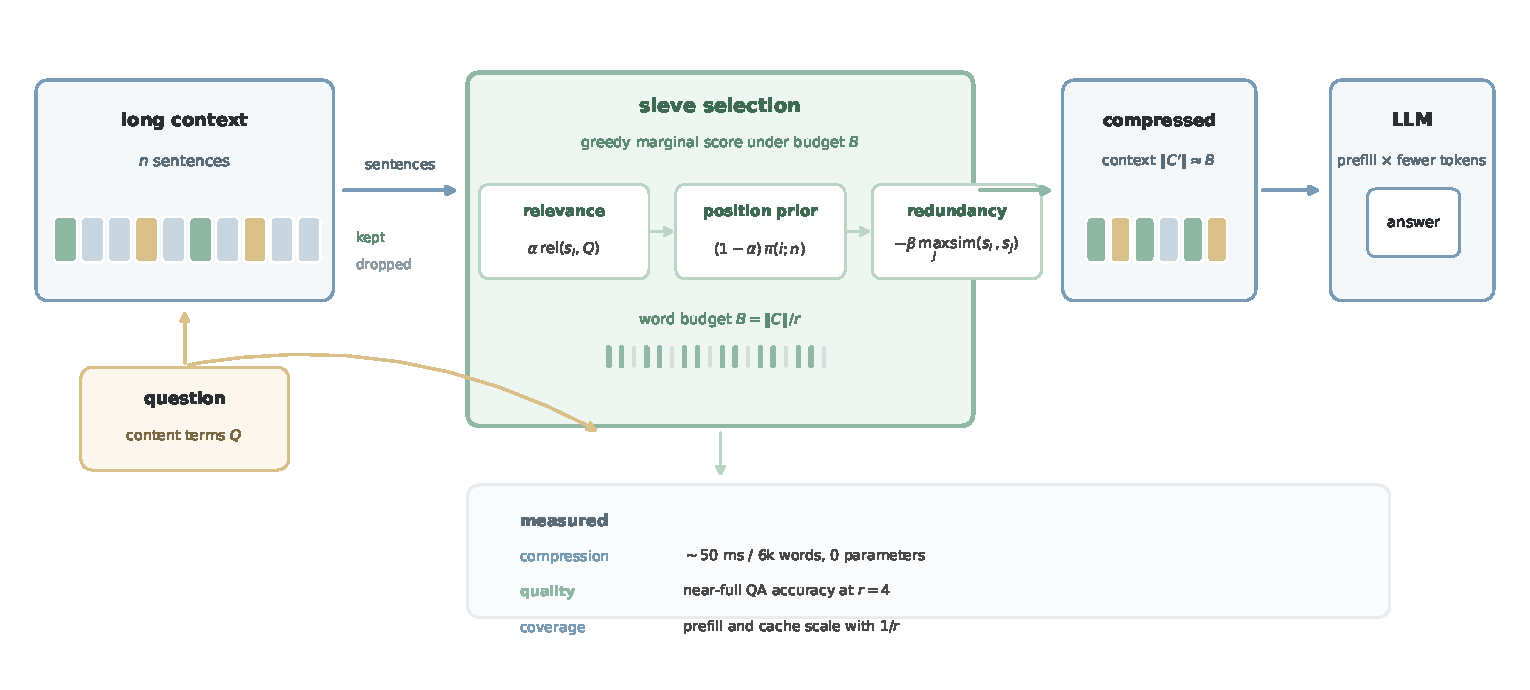
\includegraphics[width=0.98\linewidth]{figures/fig1_architecture.pdf}
\caption{The \method{} pipeline. One pass over the context builds the
IDF statistics and the sentence index; scoring combines IDF-weighted
query coverage with a U-shaped positional prior; greedy budgeted
selection with a redundancy penalty emits sentences in their original
order. No model, tokenizer, or external corpus is involved.}
\label{fig:pipeline}
\end{figure}

\subsection{Scoring}
Each sentence $s_i$ receives a base score
\begin{equation}
\label{eq:base}
\mathrm{base}_i \;=\; \alpha\,\mathrm{rel}_i \;+\; (1-\alpha)\,\pi_i,
\end{equation}
a convex combination of query relevance and a positional prior.

\paragraph{Question relevance.}
Tokenize $Q$ into content terms (lowercased, stopword-filtered). Let
$\mathrm{idf}(t)=\log\frac{n+1}{\mathrm{df}(t)+1}+1$ be the smoothed
inverse document frequency of term $t$ over the sentences of $C$
itself, so no external corpus or training set is consulted. The
relevance of $s_i$ is the IDF-weighted coverage of query terms it
contains,
\begin{equation}
\label{eq:rel}
\mathrm{rel}_i \;=\;
\frac{1}{\sqrt{\abs{s_i}}}\sum_{t \in Q \cap s_i}
\mathrm{tf}(t, Q)\,\mathrm{idf}(t),
\end{equation}
normalized by the square root of sentence length to suppress a bias
toward long sentences. Query terms are counted with saturation
$\mathrm{tf}(\cdot,Q) \in \{0, 1, 2\}$ capped at two.

\paragraph{Positional prior.}
Let $x_i = (i-1)/(n-1)\in[0,1]$ be the relative position of $s_i$. The
prior is U-shaped,
\begin{equation}
\label{eq:pos}
\pi_i \;=\; \mathrm{floor} + (1-\mathrm{floor})\,
\lvert 2x_i - 1\rvert^{\gamma},
\end{equation}
so the first and last sentences receive weight $1$ and the middle
receives $\mathrm{floor}$. The shape encodes the primacy and recency
advantage that placement studies of long-context models report
\citep{liu2023lost}; $\gamma$ controls how sharply the middle is
penalized. With $\mathrm{floor}=1$ the prior is flat and ablates away.

\subsection{Budgeted greedy selection}
The selector fills the word budget greedily. At each step it picks the
sentence maximizing marginal score
\begin{equation}
\label{eq:mmr}
\mathrm{score}(i \mid S) \;=\; \mathrm{base}_i
\;-\; \beta \max_{j \in S} \mathrm{sim}(s_i, s_j),
\end{equation}
where $S$ is the already-selected set and
$\mathrm{sim}(\cdot,\cdot)\in[0,1]$ is IDF-weighted cosine similarity
between sentence token vectors. The penalty of weight $\beta$ skips
near-duplicate sentences, which are common in the methods and
related-work sections of scientific text. Selection stops when the
budget is exhausted; the output concatenates selected sentences in
original order. Keeping order matters: the reader sees a coherent
excerpt, and the positional prior that shaped selection also shapes
what the reader finally sees. \autoref{alg:sieve} gives the complete
procedure.

\begin{algorithm}[t]
\caption{\method{} selection}
\label{alg:sieve}
\KwIn{context sentences $s_1,\dots,s_n$, question $Q$, budget $B$,
weights $\alpha,\beta,\mathrm{floor},\gamma$}
split $C$ into sentences; tokenize; build IDF statistics over
sentences\;
$\mathrm{rel}_i \leftarrow$ \eqref{eq:rel} and
$\pi_i \leftarrow$ \eqref{eq:pos} for each $i$\;
$S \leftarrow \emptyset$; $\mathrm{used} \leftarrow 0$\;
\While{$\mathrm{used} < B$}{
  $i^{*} \leftarrow \arg\max_{i \notin S}
  \mathrm{base}_i - \beta \max_{j \in S}
  \mathrm{sim}(s_i, s_j)$ \tcp*{greedy MMR step}
  \If{$\mathrm{used} + \abs{s_{i^{*}}} > B$}{
    \textbf{break} \tcp*{budget exhausted}
  }
  $S \leftarrow S \cup \{i^{*}\}$;
  $\mathrm{used} \leftarrow \mathrm{used} + \abs{s_{i^{*}}}$\;
}
\Return the sentences of $S$ in original index order
\end{algorithm}

\subsection{Configuration}
Four hyperparameters govern \method{}: $\alpha$ trades relevance
against position, $\beta$ sets the redundancy penalty, $\mathrm{floor}$
fixes the middle weight, and $\gamma$ shapes the prior. We
grid-searched $\alpha \in \{0.3, 0.6, 0.9\}$ on 20 development
examples disjoint from the test split and fixed $\beta=0.3$,
$\mathrm{floor}=0.35$, $\gamma=1.5$ without tuning. The selected
$\alpha=0.3$ leans on the positional prior, a choice the placement
analysis of \autoref{sec:robustness} is consistent with. Sensitivity
to all four values is reported in \autoref{sec:robustness}, and
(central to the generalization claim of \autoref{sec:discussion}) the
same configuration is applied unchanged to all three datasets: no
per-dataset tuning is performed anywhere in this paper.

\section{Theoretical analysis}
\label{sec:theory}
This section states what the design guarantees and what it
deliberately does not. Proofs are short and appear in
\autoref{app:proofs}; the interest is in making the assumptions
explicit, because the empirical sections then measure how far real
benchmarks satisfy them.

\subsection{Cost: one arithmetic pass, no hosted model}
\begin{proposition}[Cost of \method{}]
\label{prop:cost}
Let $W$ be the context word count, $n$ the number of sentences, $k$
the number selected, and $\bar{s}$ the mean sentence length in tokens.
Segmentation, tokenization, and IDF construction take $O(W)$
elementary word-level operations; relevance and the prior take
$O(W + n\abs{Q})$; the greedy loop takes $O(k\,n\,\bar{s})$ in the
worst case, each step dominated by sparse-counter similarity
evaluations. Peak memory is the token counters of the input. No
parameter, model, or external corpus is consulted:
$c_{\mathrm{host}} = 0$.
\end{proposition}

The proof is immediate from the algorithm: each preprocessing stage
touches each token a constant number of times, and the greedy loop
performs at most $k$ passes over $n$ candidates whose similarity
evaluation costs $O(\bar{s})$ on sparse counters. At the operating
point of our experiments ($W \approx 6{,}000$, $n \approx 300$,
$k \approx 75$) the bound is a few million elementary operations,
against a measured \TimeSieSixk\,\ms{} on one CPU core of the
evaluation container (\autoref{sec:efficiency}). The greedy stage, not
the preprocessing, dominates at this operating point, which is why we
state the two terms separately rather than call the whole selector
linear.

\begin{proposition}[Floor of scorer-based compression]
\label{prop:floor}
Any compressor that scores the context with a model $M_s$ of
$\abs{M_s}$ parameters over $L$ context tokens performs at least
$2\abs{M_s} L$ FLOPs per compression call, before any budget search
that repeats the pass, and incurs $c_{\mathrm{host}} \ne 0$.
\end{proposition}

This is the standard forward-pass FLOP count \citep{kaplan2020scaling}.
For GPT-2-small ($\abs{M_s} = 124$M) at $L \approx 8{,}000$ tokens,
the floor is $1.98 \times 10^{12}$ FLOPs: at least five orders of
magnitude above \method{}'s arithmetic bound at the same context, and
the floor does not include hosting, tokenization matched to the
scorer, or the coarse-to-fine repetitions that budget searches add.
\autoref{sec:efficiency} measures both sides on identical hardware
rather than leaving the comparison at the FLOP level.

\subsection{Selection: what question conditioning guarantees}
\label{sec:guarantees}
We now state the condition under which relevance scoring provably
recovers evidence, and contrast it with truncation. The condition is
about the instance, not the method.

\begin{condition}[Lexical coverage]
\label{cond:lexical}
Instance $(C, Q, E)$ satisfies lexical coverage if every gold
evidence sentence weakly dominates every non-evidence sentence in
IDF-weighted query coverage:
$\mathrm{rel}(e) \ge \mathrm{rel}(s)$ for all $e \in E$,
$s \in C \setminus E$.
\end{condition}

\begin{proposition}[Recall of relevance-only selection]
\label{prop:relonly}
Under \autoref{cond:lexical}, if the budget satisfies
$B \ge \sum_{e \in E} \abs{e}$, then relevance-only selection
($\alpha=1$, flat prior, $\beta=0$) attains evidence recall $\rho=1$:
every evidence sentence is selected before any non-evidence sentence
it dominates, and all fit within $B$.
\end{proposition}

\begin{proposition}[Recall of head truncation]
\label{prop:head}
Let the position of each gold evidence sentence be uniform on
$\{1, \ldots, n\}$ and independent across sentences, and let
truncation keep the prefix of $\lceil n/r \rceil$ sentences. Then the
expected evidence recall is
$\mathbb{E}[\rho_{\mathrm{head}}] = \min(1, 1/r)$.
\end{proposition}

Two readings follow. First, the separation between question-conditioned
and question-agnostic selection grows linearly in $r$: under
\autoref{cond:lexical} with sufficient budget the gap is $1 - 1/r$,
which is 50 points at $r=2$, 75 at $r=4$, and 94 at $r=16$. This is
exactly the shape the ratio sweeps of \autoref{sec:results} measure on
all three datasets. Second, the condition is strong, and real data
satisfies it only partially: paraphrased evidence, distractors that
share query terms, and multi-hop questions whose terms spread across
sentences all violate it. The ablations of \autoref{sec:ablation}
quantify the departure: relevance-only recall on QASPER is well below
the $\rho = 1$ of the idealized condition; and \autoref{sec:discussion}
measures how the departure varies by dataset. The propositions are
not claims that \method{} is optimal; they are the mechanism, stated
precisely enough to be falsified. They also delimit what BM25 can
claim: BM25 is a relevance-only selector up to term saturation and
length normalization, so \autoref{prop:relonly} is the guarantee it
approximates, and \autoref{prop:cost} does not apply to it (BM25 is
likewise model-free), which is why the empirical sections measure BM25
rather than bound it.

\subsection{The positional prior as a reliability allocation}
The prior of \eqref{eq:pos} is not selected to maximize recall;
\autoref{sec:ablation} shows flat priors recall more. It allocates the
selection's reliability budget to the positions where readers attend
most reliably. If reader accuracy in using a retained sentence is a
U-shaped function $u(x)$ of its position $x$, as placement studies
report \citep{liu2023lost}, then a selector that must discard
sentences maximizes expected usable evidence by discarding from the
middle first, which is what the prior does: with
$\mathrm{floor} < 1$, middle sentences enter the budget only after
end-position sentences of comparable base score. The cost is explicit
and measured in \autoref{sec:robustness}: when the only evidence copy
sits mid-document, the prior discards it. The design treats selector
recall and reader reliability as exchangeable under a stated profile
rather than optimizing either alone, and the $\mathrm{floor}$
hyperparameter exposes the exchange rate to the deployer. BM25, which
lacks the prior, occupies the opposite end of this exchange: maximal
raw recall, no placement control. Which end a deployment should choose
is an empirical question the end-task protocol addresses.

\subsection{What the design does not guarantee}
Three limits are worth stating before the measurements, because the
measurements confirm all three. \emph{Lexical reach}:
\autoref{cond:lexical} fails outright for paraphrased or multilingual
evidence, and IDF weights numbers and code identifiers crudely.
\emph{Budget tightness}: when
$B < \sum_{e \in E} \abs{e}$ no selector attains $\rho = 1$, and the
ratio sweep measures how each degrades. \emph{Reader variance}:
end-task quality couples the selector to the reader's own positional
profile, which the selector models only through the borrowed U-shape;
our reader-side placement profile is taken from prior work rather than
re-measured, a scope limitation \autoref{sec:limitations} returns to.

\section{Experimental setup}
\label{sec:exp}

\subsection{Benchmarks and pools}
\label{sec:pools}
We use three benchmarks, chosen because each annotates the gold
evidence, which the reader-free protocol of \autoref{sec:protocols}
requires, and because together they span abstract and entity-named
question styles. Long-context suites without evidence annotations
(LongBench \citep{bai2023longbench}, MuSiQue \citep{trivedi2022musique}
in its distractor form) cannot support the recall protocol and are
therefore out of scope for the selector-level claims.

\paragraph{QASPER.}
QASPER \citep{dasigi2021qasper} contains information-seeking questions
over full NLP papers. From the train split's paper-level records we
select questions whose gold answers are extractive spans, short
free-form strings, or yes/no judgments, cap each context at 6{,}000
words (the cap binds on papers that exceed it), and keep records whose
annotated evidence sentences are locatable in the segmented context.
The resulting recall pool contains \NRecQ{} records (median
\PoolQMedWords{} words, 90th percentile 5{,}576), from which the
end-task test split of 25 examples and the 20-example development
split are drawn disjointly and fixed by seed before any test
evaluation; the development split mixes ten QASPER with ten HotpotQA
distractor records for tuning diversity, while the test split is
QASPER only. The official QASPER test labels are not public, which is
why all held-out sampling comes from the train split.

\paragraph{HotpotQA.}
HotpotQA \citep{yang2018hotpotqa} in the distractor setting pairs each
question with ten paragraphs, two of which contain the supporting
facts. We flatten the paragraphs into a single context under the same
6{,}000-word cap and keep records whose supporting-fact sentences are
locatable. The recall pool contains \NRecH{} records (median 888
words).

\paragraph{2WikiMultihopQA.}
2WikiMultihopQA \citep{ho2020wiki} builds compositional comparison and
inference questions over Wikipedia with annotated reasoning chains.
The same flattening and locatability protocol yields a pool of
\NRecW{} records (median 602 words). Its dev split provides the
examples; no test labels are used.

The three pools total \TotalRecords{} records. All are processed by
the same segmenter, the same locatability rule (evidence sentence
prefix-matches a context sentence), and the same word-budget
convention; no per-dataset tuning of any kind is performed.

\subsection{Reader and decoding}
All end-task conditions use the same reader: GLM-4-Plus served through
its public API \citep{glm2024chatglm}, temperature $0$, maximum 96
answer tokens, and a fixed instruction to answer with the shortest
span from the context or yes/no. The reader sees only the compressed
(or full) context and the question. We record the served token counts
of every call. End-task evaluation is scoped to the QASPER test split
at the $4\times$ operating point; the selector-level protocols carry
the multi-dataset claims.

\subsection{Baselines}
\label{sec:baselines}
All selectors share \method{}'s word-budget convention so that the
comparison isolates the selection rule. Full context uses $C$
unchanged. Head truncation keeps the first $B$ words. Random selects
sentences uniformly under the budget with two seeds. Stride keeps
every $k$-th sentence with $k$ chosen to meet the budget. TextRank
\citep{mihalcea2004textrank} ranks sentences by PageRank on an
IDF-weighted cosine graph and packs the top-ranked sentences under the
budget; it is the strongest model-free summarizer that does not see
the question.

\paragraph{BM25 sentence ranking.}
BM25 \citep{robertson2009bm25} is the classical question-conditioned
baseline: the question is the query, each sentence is a document, IDF
is smoothed over the sentences of the context itself (matching
\method{}'s corpus-local statistics), and the top-ranked sentences are
packed under the same budget and emitted in original order. It is the
strongest question-aware, model-free comparator and the reference
point that any selector machinery beyond relevance ranking
(positional priors, redundancy penalties, greedy marginal search)
must justify. We run it on all three pools at every ratio.

\paragraph{GPT-2 perplexity gate (neural baseline).}
To compare against the neural compressors on measured terms, we
implement the perplexity gate of LLMLingua-style compression
\citep{jiang2023llmlingua} at sentence granularity, the same output
granularity as \method{}, so the comparison isolates the scorer and
not the unit. The scorer is GPT-2 small (124M parameters)
\citep{radford2019gpt2}, dynamically quantized to int8. For each
record, one forward pass scores every sentence by the mean negative
log-likelihood of its tokens, with the question prepended to the
first window so the gate is question-conditioned in the LongLLMLingua
sense \citep{jiang2023longllmlingua}; sentences are packed into at
most 1{,}024-token windows of whole sentences, which is GPT-2's
position limit. Selection keeps the lowest-perplexity sentences under
the same budget and preserves order. The pass is the floor of what
any scorer-based compressor pays; coarse-to-fine budget searches
repeat it. We run the gate on \GateN{} QASPER records (the first
\GateN{} of the recall pool, a fixed prefix) and measure its scoring
latency on the same container as every other timing number in this
paper. We do not run LLMLingua-2's distilled token classifier: its
checkpoint requires hosting a different architecture, and the GPT-2
gate already represents the mechanism and the cost floor of that
family; \autoref{sec:limitations} returns to what that comparison
cannot claim.

\subsection{Metrics and statistics}
We report exact match (EM) and token-level F1 with SQuAD-style
normalization \citep{yang2018hotpotqa} against gold answers, plus the
percentage of full-context F1 retained by each compressor. For the
selector protocol we report evidence recall at matched budgets.
Uncertainty is a percentile bootstrap over records with 1{,}000
resamples, reported as 95\% intervals on the means, together with
paired bootstrap intervals for the \method{}-versus-baseline
differences per dataset; the random baseline additionally reports the
standard deviation across two selection seeds. Timing numbers are
medians of five runs after one warm-up (three for the gate). The
recall and end-task protocols are never pooled: where both appear,
their sample sizes are stated separately.

\subsection{Implementation and compute}
The selector is a single Python module with NumPy as its only
dependency beyond the standard library. All journal-version
experiments ran in a container with 2 vCPUs and 4 GB of memory; the
GPT-2 gate ran in the same container on the same cores (int8, two
threads), so every latency comparison in \autoref{sec:efficiency} is
same-hardware. No GPU was used for any measurement reported in this
paper; the A100 floor for the gate is analytic, computed from
$2\abs{M_s} L$ FLOPs at 40\% utilization, and the projection of
\autoref{sec:projection} is likewise analytical with stated
assumptions. The repository regenerates every table and figure from
raw checkpoints with one command per artifact.

\section{Main results}
\label{sec:results}

\subsection{End-task question answering at \texorpdfstring{$4\times$}{4x}}
\label{sec:qa}

\begin{table}[t]
\centering
\caption{Question answering at a $4\times$ compression on the QASPER
test split ($n{=}\QAN$ per method after exclusions, see
\autoref{sec:pools}), reader GLM-4-Plus at temperature 0. EM and
token-level F1 in percent; brackets are bootstrap 95\% intervals;
$\Delta$F1 is the gap to full context. Prompt tokens are the served
means. \method{} and truncation overlap; the question-agnostic
selectors cluster below. The end-task sample is small and its claims
are scoped accordingly in the text. The GPT-2 gate was not run under
this protocol; it is compared under the selector protocol
(\autoref{sec:recall}, \autoref{sec:efficiency}).
\ifdefined\QABmF{}BM25 is included under this protocol.\else{}BM25
was not run under this protocol either; it is compared under the
selector protocol, and the released expansion script covers it end
to end.\fi{}}
\label{tab:qa}
\small
\begin{tabular}{lccccc}
\toprule
Method & EM $\uparrow$ & F1 $\uparrow$ & $\Delta$F1 & Retain &
prompt tokens \\
\midrule
Full context & \QAFullEM{} & \textbf{\QAFullF} & -- & 100\% &
\QAFullTok \\
\midrule
Head & \QAHeaEM{} & \textbf{\QAHeaF} & \QAHeaDelta{} &
\QAHeaRetain\% & \QAHeaTok \\
Random & \QARanEM{} & \QARanF{} & \QARanDelta{} & \QARanRetain\% &
\QARanTok \\
Stride & \QAStrEM{} & \QAStrF{} & \QAStrDelta{} & \QAStrRetain\% &
\QAStrTok \\
TextRank & \QATREM{} & \QATRF{} & \QATRDelta{} & \QATRRetain\% &
\QATRTok \\
BM25 & \QAorDash{Bm}{EM} & \QAorDash{Bm}{F} & \QAorDash{Bm}{Delta} &
\QARetainOrDash{Bm} & \QAorDash{Bm}{Tok} \\
\method{} & \QASieEM{} & \QASieF{} & \QASieDelta{} & \QASieRetain\% &
\QASieTok \\
\bottomrule
\end{tabular}
\end{table}

\autoref{tab:qa} reports the end-task comparison at $r=4$ on the test
split. Three observations. First, every compressor loses accuracy
relative to the full context, and the loss is large: the full-context
interval is wide at $n{=}\QAN$, but its point estimate (\QAFullF{} F1)
sits well above every compressed condition, which is the expected
price of removing three quarters of the context. Second, \method{} and
head truncation cannot be separated at this sample size in either
direction: the paired bootstrap interval for the F1 difference is
[\QAPairSHLo, \QAPairSHHi], with point estimate \QAPairSH{} points. On
questions about a paper's overall setup, the evidence often sits in
the opening sections, which is the regime where a fixed prefix is
already competent. Third, the question-agnostic selectors sit below
\method{} in point estimate (paired differences of \QAPairSTR{} points
against TextRank and \QAPairSRan{} against random selection), though
these intervals also include zero at $n{=}\QAN$; the sample is too small
to separate end-task orderings among the compressors, and we report
the point estimates with that caveat rather than claim separations the
design cannot resolve.
\ifdefined\QAPairSBm Against the question-conditioned lexical
baseline the paired interval is
[\QAPairSBmLo, \QAPairSBmHi] (point estimate \QAPairSBm{} points).
\fi{} The end-task picture is therefore that
\method{} matches the strongest cheap baseline at this operating point
on this benchmark. Where the question actually matters, the picture
sharpens at the scale the selector protocol can afford, which is the
subject of the next two subsections.

\subsection{Evidence retention at scale: three datasets}
\label{sec:recall}

\begin{table}[t]
\centering
\caption{Gold evidence sentence recall at a $4\times$ budget under the
reader-free protocol (no LLM calls; brackets are bootstrap 95\%
intervals over records). \method{} uses the same configuration on all
three datasets. $\Delta$ rows are paired 95\% intervals for the
difference in recall points. BM25 is the question-conditioned,
model-free reference; the question-agnostic selectors cluster far
below.}
\label{tab:recall}
\small
\begin{tabular}{lccc}
\toprule
 & QASPER ($n{=}\NRecQ$) & HotpotQA ($n{=}\NRecH$) &
2Wiki ($n{=}\NRecW$) \\
\midrule
\method{} &
\textbf{\RecQSie} [\RecQSieLo, \RecQSieHi] &
\textbf{\RecHSie} [\RecHSieLo, \RecHSieHi] &
\textbf{\RecWSie} [\RecWSieLo, \RecWSieHi] \\
BM25 &
\RecQBm{} [\RecQBmLo, \RecQBmHi] &
\RecHBm{} [\RecHBmLo, \RecHBmHi] &
\RecWBm{} [\RecWBmLo, \RecWBmHi] \\
Head &
\RecQHea{} [\RecQHeaLo, \RecQHeaHi] &
\RecHHea{} [\RecHHeaLo, \RecHHeaHi] &
\RecWHea{} [\RecWHeaLo, \RecWHeaHi] \\
Random &
\RecQRan{} [\RecQRanLo, \RecQRanHi] &
\RecHRan{} [\RecHRanLo, \RecHRanHi] &
\RecWRan{} [\RecWRanLo, \RecWRanHi] \\
Stride &
\RecQStr{} [\RecQStrLo, \RecQStrHi] &
\RecHStr{} [\RecHStrLo, \RecHStrHi] &
\RecWStr{} [\RecWStrLo, \RecWStrHi] \\
TextRank &
\RecQTR{} [\RecQTRLo, \RecQTRHi] &
\RecHTR{} [\RecHTRLo, \RecHTRHi] &
\RecWTR{} [\RecWTRLo, \RecWTRHi] \\
\midrule
$\Delta$ (\method{}$-$Head) &
[\PairQSHLo, \PairQSHHi] &
[\PairHSHLo, \PairHSHHi] &
[\PairWSHLo, \PairWSHHi] \\
$\Delta$ (\method{}$-$BM25) &
[\PairQSBmLo, \PairQSBmHi] &
[\PairHSBmLo, \PairHSBmHi] &
[\PairWSBmLo, \PairWSBmHi] \\
\bottomrule
\end{tabular}
\end{table}

\autoref{tab:recall} is the paper's central selector-level result, and
the conference version's single-dataset finding survives the scaling
intact and sharpened. On QASPER at $n{=}\NRecQ$, \method{} retains
\RecQSie\% of the annotated evidence against \RecQHea\% for head
truncation, and the intervals, which at the conference version's
$n=191$ only touched at their edges, are now separated, with the
paired difference at \PairQSH{} points [\PairQSHLo, \PairQSHHi]. On
HotpotQA the margin more than triples: \RecHSie\% against
\RecHHea\%, a paired difference of \PairHSH{} points
[\PairHSHLo, \PairHSHHi]. On 2WikiMultihopQA the margin is
\PairWSH{} points [\PairWSHLo, \PairWSHHi]. Every question-agnostic
selector sits below \method{} on every dataset, and every paired
interval excludes zero by a wide margin.

The BM25 rows give the table its second axis, and the finding is
reported as measured: BM25 retains \emph{more} raw evidence than the
full \method{} configuration on all three datasets, by
$\abs{\PairQSBm}$ paired points on QASPER [\PairQSBmLo, \PairQSBmHi],
\PairHSBm{} on HotpotQA, and \PairWSBm{} on 2WikiMultihopQA. The
result is not an anomaly but the direct empirical counterpart of
\autoref{prop:relonly}: BM25 is relevance ranking distilled, and
relevance ranking is exactly the term of \method{} that recovers
evidence. The selector's own ablations (\autoref{sec:ablation}) say
the same thing from the inside: flattening the positional prior
raises \method{}'s recall from \AblSie\% to \AblNoPos\%, and stripping
the selector to relevance alone reaches \AblRelOnly\%, within a point
of BM25's \RecQBm\%. What BM25 and the relevance-only ablation give up
is the subject of the placement analysis (\autoref{sec:robustness}):
retained evidence concentrated where readers attend least reliably,
and no redundancy control under tight budgets. The end-task protocol,
not the recall protocol, is where that trade is decided, and
\autoref{sec:corr} measures how loosely the two protocols are
connected.

Two regularities in the table deserve emphasis. First, head
truncation lands at 22--31\% recall on all three datasets, close to
the $1/r = 25\%$ that \autoref{prop:head} predicts for uniformly
placed evidence, and \autoref{sec:discussion} confirms that evidence
positions are close to uniform on all three pools. The prediction is
not a strawman: it is what a fixed prefix mechanically achieves, and
the measured agreement is a useful validation that the recall protocol
measures what it claims. Second, \method{}'s margin over the
question-agnostic selectors differs by dataset, and the ordering
tracks the lexical signal in the question. HotpotQA and
2WikiMultihopQA questions name the entities whose sentences carry the
answer, so IDF-weighted coverage fires strongly; QASPER's questions
are more often abstract (what, how, why), so the signal is weaker and
the margin smaller. The same \method{} configuration is used
throughout; the datasets, not the method, vary.

\subsection{Evidence retention under increasing compression}
\label{sec:ratio}

\begin{figure}[t]
\centering
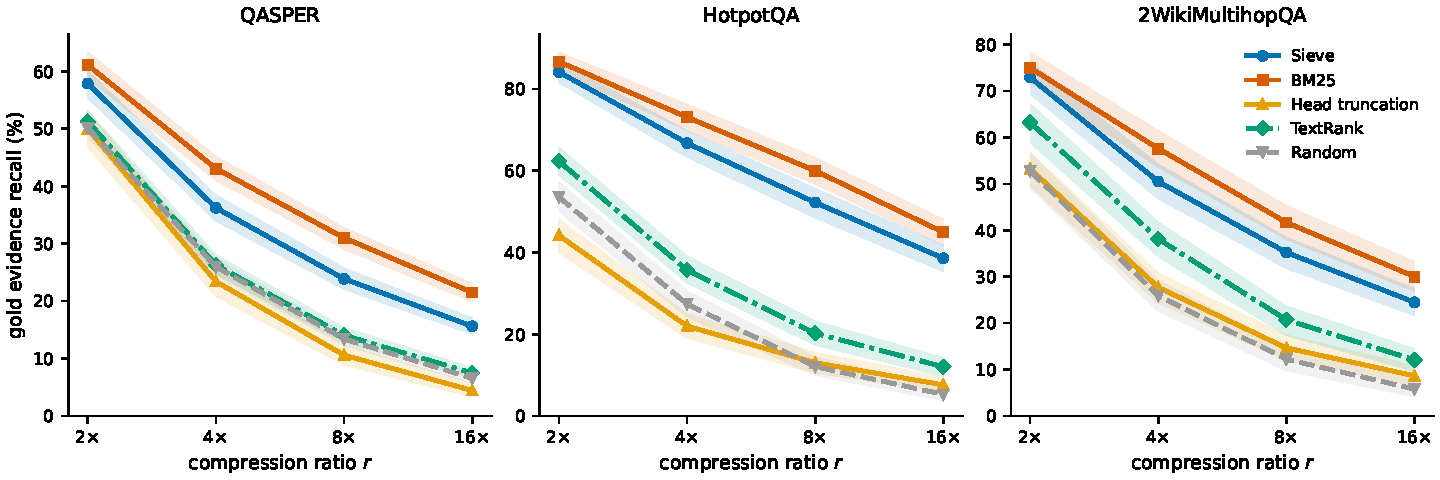
\includegraphics[width=0.98\linewidth]{figures/fig2_ratio3.pdf}
\caption{Gold evidence sentence recall as a function of the
compression ratio $r$ at matched word budgets, one panel per dataset
(shaded regions are bootstrap 95\% intervals). The pattern is the same
on all three: truncation is competitive at $r=2$ and collapses as the
budget tightens; the question-conditioned selectors (\method{}, BM25)
degrade far more slowly; and the gap over every question-agnostic
selector is separated by the intervals from $r=4$ onward.}
\label{fig:ratio}
\end{figure}

\autoref{fig:ratio} sweeps the budget from $r=2$ to $r=16$ under the
evidence-recall protocol on all three pools. The qualitative pattern
from the conference version's single dataset replicates on the two
additions, and BM25 tracks it from above. At $r=2$, every method
retains most of the evidence and the compressors are within noise of
one another (\RatQSieTwo{} for \method{} against \RatQHeaTwo{} for
truncation and \RatQBmTwo{} for BM25 on QASPER; \RatHSieTwo{} against
\RatHHeaTwo{} on HotpotQA). The separation grows as the budget
tightens. On QASPER at $r=8$, \method{} retains \RatQSieEight\% of the
annotated evidence against \RatQHeaEight\% for truncation and
\RatQTREight{} for TextRank, with BM25 at \RatQBmEight{}; on HotpotQA
the same ratio is \RatHSieEight{} against \RatHHeaEight{}; on
2WikiMultihopQA \RatWSieEight{} against \RatWHeaEight{}. At $r=16$
the gaps reach \RatQSieSixteen{} against \RatQHeaSixteen{} on QASPER
and \RatHSieSixteen{} against \RatHHeaSixteen{} on HotpotQA, with
non-overlapping intervals throughout. The mechanism is the design
intent, now confirmed across datasets: relevance scoring keeps pulling
question-covering sentences out of the whole document while a fixed
prefix shrinks into the first quarter of the text, and the same
mechanism that is interchangeable at generous budgets dominates at
tight ones, where compression actually matters. This is the empirical
shape of \autoref{prop:relonly} and \autoref{prop:head}: the gap grows
in $r$ as the propositions predict, though the absolute level of
every method's recall stays below the idealized $\rho=1$ of
\autoref{cond:lexical}, by an amount that measures how far real
benchmarks satisfy lexical coverage.

\section{Ablation study}
\label{sec:ablation}

\begin{table}[t]
\centering
\caption{Selector-level ablations: evidence recall of \method{}
variants at $r=4$ on the QASPER recall pool ($n=\NRecQ$; the same
protocol as \autoref{tab:recall}), with BM25 as the external
relevance-ranking reference. Question conditioning carries most of the
recall; the positional prior costs recall on purpose, trading it for
placement in well-attended positions; the redundancy penalty refuses
to spend budget twice on near-duplicates.}
\label{tab:ablation}
\small
\begin{tabular}{lc}
\toprule
Configuration & evidence recall $\uparrow$ \\
\midrule
\method{} (full) & \AblSie \\
BM25 (external reference) & \RecQBm \\
\midrule
no question conditioning ($\alpha=0$) & \AblNoQ \\
flat positional prior ($\mathrm{floor}=1$) & \AblNoPos \\
no redundancy penalty ($\beta=0$) & \AblNoRed \\
relevance only ($\alpha=1$, flat, $\beta=0$) & \AblRelOnly \\
\bottomrule
\end{tabular}
\end{table}

\autoref{tab:ablation} removes one component at a time on the expanded
QASPER pool; the ordering matches the conference version's $n=191$
analysis, now with intervals an order of magnitude tighter at
$n{=}\NRecQ$. Removing question conditioning drops recall from
\AblSie\% to \AblNoQ\%, the single largest factor: without the query
the score rewards generally informative sentences, and evidence for a
specific question is not the same as salient text. This is the
component-to-claim mapping for the multi-dataset result of
\autoref{tab:recall}: the margin over question-agnostic selectors is
the measured value of the question, and it is largest where questions
are entity-named. The redundancy penalty is recall-neutral at this
ratio (\AblNoRed\% against \AblSie\%): its work is diversity under
tight budgets, refusing to spend scarce budget twice on near-duplicate
sentences, which are common in the methods and related-work sections
of scientific text.

The two remaining rows are the table's most instructive finding, and
BM25 now makes it legible from the outside as well as the inside. A
relevance-only configuration (question conditioning with a flat prior
and no penalty) reaches \AblRelOnly\% recall, the highest number in
the table, and BM25, an entirely external implementation of
relevance ranking, lands at \RecQBm\%, within a point of it. The
agreement is the point: the relevance term, implemented either way,
is a near-oracle for evidence \emph{recovery} under
\autoref{cond:lexical}, and everything \method{} adds on top of it is
a deliberate trade of raw recall for other objectives. The positional
prior behaves differently, and the difference is instructive:
flattening the prior raises recall from \AblSie\% to \AblNoPos\%; the
U shape actively deprioritizes middle sentences, and when the only
evidence copy sits there the prior discards it. The same U shape,
however, places retained evidence where readers attend most reliably,
which is the trade-off \autoref{sec:theory} formalized as a
reliability allocation and \autoref{sec:robustness} measures position
by position. The component ablations and the multi-dataset results
compose into a single account of when \method{} wins: the margin over
question-agnostic selection scales with the strength of the lexical
signal (\autoref{cond:lexical} of \autoref{prop:relonly}), the prior
converts part of it into placement, and both terms are visible in
\autoref{tab:recall} as the dataset-dependent gap over
question-agnostic selection, and in the BM25 rows as the price of
the prior.

\section{Efficiency analysis}
\label{sec:efficiency}
This section reports the cost axis of the trade-off for every method,
on identical hardware, and assembles the pieces into the frontier
picture that the introduction advertised.

\subsection{Compression latency}
\label{sec:latency}

\begin{figure}[t]
\centering
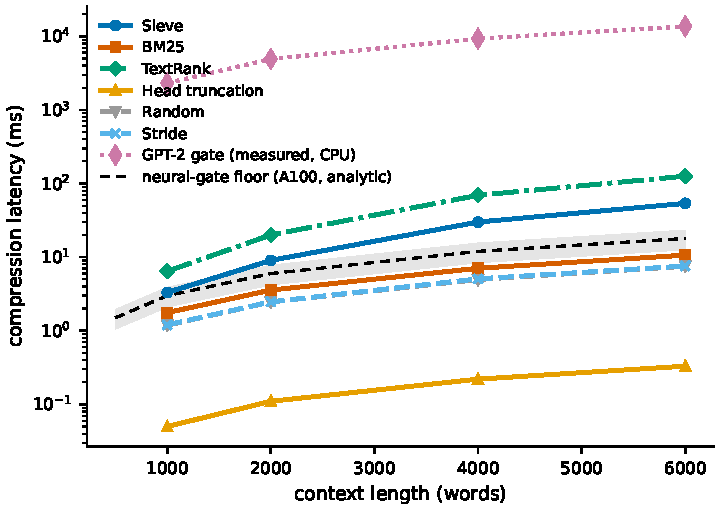
\includegraphics[width=0.72\linewidth]{figures/fig3_cost.pdf}
\caption{Measured compression latency versus context length on the
evaluation container (median of 5 runs; 3 for the gate; same box as
every other measured number in this paper). The dashed band is the
analytic wall-clock of one served forward pass of a 124M-parameter
scorer over the full context on an A100 at 40\% utilization, the
minimum any perplexity-gated compressor must pay; coarse-to-fine
pipelines repeat this pass at every budget iteration. The statistical
selectors sit at or below the band with no model hosted; the measured
CPU points for the GPT-2 gate (dotted) lie three orders of magnitude
above it.}
\label{fig:cost}
\end{figure}

\autoref{fig:cost} compares the measured compression cost of the
statistical selectors (\method{}, BM25, TextRank, random, stride,
and head truncation) across context lengths, and against the floor
of perplexity-gated compression: one served forward pass of the
GPT-2-scale scorer \citep{radford2019gpt2} over the full context.
\method{} compresses a 6{,}000-word context in \TimeSieSixk\,\ms{} on
the evaluation container's cores, against \TimeTRSixk\,\ms{} for
TextRank, \TimeBmSixk\,\ms{} for BM25, and \TimeHeaSixk\,\ms{} for
truncation; BM25 is the cheapest question-conditioned selector in the
study, running at roughly \BmSpeedup$\times$ the speed of the full
\method{} at the same length, a direct consequence of skipping the
greedy marginal search. Every statistical selector's cost is noise at
serving scale: the median reader call in the end-task experiment takes
\QAReaderMs\,\ms, an order of magnitude above the compression itself,
and the projection of \autoref{sec:projection} shows what the saved
prefill and cache are worth at deployment scale.

\subsection{The neural gate, measured}
\label{sec:gate}
The conference version could only bound the neural compressor's cost
analytically; this version measures it. The GPT-2 perplexity gate of
\autoref{sec:baselines} runs on the same container, the same cores,
and the same records as every other method. Three facts come out of
the measurement. First, the gate's scoring pass costs
\GateLatMedS\,s of CPU time per median context (\GateMedWords{} words;
\GateLatPnineS\,s at the 90th percentile), and \GateLatSixkS\,s on the
\GateSixkN{} records near the 6{,}000-word cap, against \method{}'s
\TimeSieSixk\,\ms{} at the same length: roughly
\GateSieRatioSixk$\times$ more measured work for the scoring step
alone at the 6{,}000-word operating point, and
\GateSieRatioMed$\times$ at the median context. Second, even granting
the gate a GPU, the analytic A100 floor for the same pass is
\GateAOneFloorMs\,\ms{} at the median context's token count
(\GateMedTok{} tokens), at best comparable to \method{}'s entire CPU
wall-clock; and the floor assumes the scorer is already resident,
excludes tokenization and budget iterations, and prices the accelerator
that \method{} does not have at zero. Third, the gate's quality at
$4\times$ on QASPER is \GateRecall\% evidence recall
[\GateRecallLo, \GateRecallHi] against \method{}'s \RecQSie\%
[\RecQSieLo, \RecQSieHi]: on this benchmark the floor-cost
configuration of the neural approach does not beat the statistical
selector even on the reader-free metric, because GPT-2 perplexity is
a proxy for predictability, not for question relevance: the gate keeps
sentences the language model finds likely, which is not the same as
sentences that answer the question. A stronger scorer (a fine-tuned
reranker, or LLMLingua-2's distilled classifier) would be expected to
close and pass \method{} on quality, at the same or larger hosted
cost; the frontier statement of \autoref{sec:frontier} covers both
cases, and \autoref{sec:limitations} states explicitly that the gate
is the family's cost floor, not its best quality.

\subsection{The accuracy--compression--cost trade-off}
\label{sec:threeway}

\begin{table}[t]
\centering
\caption{The three-way trade-off at $r=4$ on QASPER, one row per
method; recall is the selector protocol (evidence recall at $4\times$,
$n{=}\NRecQ$), F1 the end-task protocol ($n{=}\QAN$), and latency the
measured CPU cost of the compression itself on a 6{,}000-word context
on the same container. The GPT-2 gate was not run under the end-task
protocol; its GPU floor is analytic ($2\abs{M_s} L$ FLOPs at 40\%
utilization on an A100).}
\label{tab:threeway}
\small
\begin{tabular}{lcccccc}
\toprule
Method & extra model & GPU & recall $\uparrow$ & F1 $\uparrow$ &
latency (CPU) & GPU floor \\
\midrule
Full context & -- & no & -- & \QAFullF & 0\,\ms & -- \\
Head & -- & no & \RecQHea & \textbf{\QAHeaF} & \TimeHeaSixk\,\ms & -- \\
Random & -- & no & \RecQRan & \QARanF & \TimeRanSixk\,\ms & -- \\
Stride & -- & no & \RecQStr & \QAStrF & \TimeStrSixk\,\ms & -- \\
TextRank & -- & no & \RecQTR & \QATRF & \TimeTRSixk\,\ms & -- \\
BM25 & -- & no & \textbf{\RecQBm} & \QAorDash{Bm}{F} & \TimeBmSixk\,\ms & -- \\
\method{} & -- & no & \RecQSie & \QASieF & \TimeSieSixk\,\ms & -- \\
GPT-2 gate & 124M (int8) & yes & \GateRecall & -- &
\GateLatSixkS\,s & \GateAOneFloorMs\,\ms$^{\dagger}$ \\
\bottomrule
\end{tabular}

\smallskip
{\footnotesize $^{\dagger}$analytic, at the median context's token
count; the gate's measured latency row is the 6{,}000-word operating
point (mean over the \GateSixkN{} pool records at that length).}
\end{table}

\autoref{tab:threeway} assembles the three axes. Reading it as the
formulation of \autoref{sec:tradeoff} suggests: within the model-free
rows, \method{} dominates Random, Stride, and TextRank on quality
(separated recall intervals on all three datasets) at latency within
two orders of magnitude of truncation; BM25 dominates \method{} on
raw recall at a fifth of its latency, and the two are the
complementary question-conditioned points whose trade the placement
analysis prices; and no model-free method dominates the
question-conditioned pair on any dataset at any ratio we measure. The
gate row shows what the neural corner buys and costs at its floor
configuration: its recall on QASPER is \GateRecall\% against
\method{}'s \RecQSie\% (a deficit of
\RecQSie{}$-$\GateRecall{} points with separated intervals; the gate
also does not separate from head truncation at \RecQHea\%), and its
cost is a hosted 124M-parameter model, a matched tokenizer, and
roughly \GateSieRatioSixk$\times$ more measured CPU work at the
6{,}000-word operating point, or an accelerator whose analytic floor
already matches \method{}'s entire CPU budget. The table is the
paper's answer to the question a practitioner actually asks: what
does conditioning on the question cost, and what does a neural scorer
buy over not hosting one? On these benchmarks the answer is:
conditioning on the question is nearly free and worth tens of recall
points over question-agnostic selection; relevance ranking alone
(BM25) already captures most of that gain at the lowest
question-aware latency; the floor-cost neural scorer, at this scale,
does not even match truncation on recall, let alone buy back its own
cost; and the quality that larger scorers would add is bought at
hosted-model cost that the frontier of \autoref{sec:frontier} makes
explicit.

\subsection{The accuracy--efficiency frontier}
\label{sec:frontier}

\begin{figure}[t]
\centering
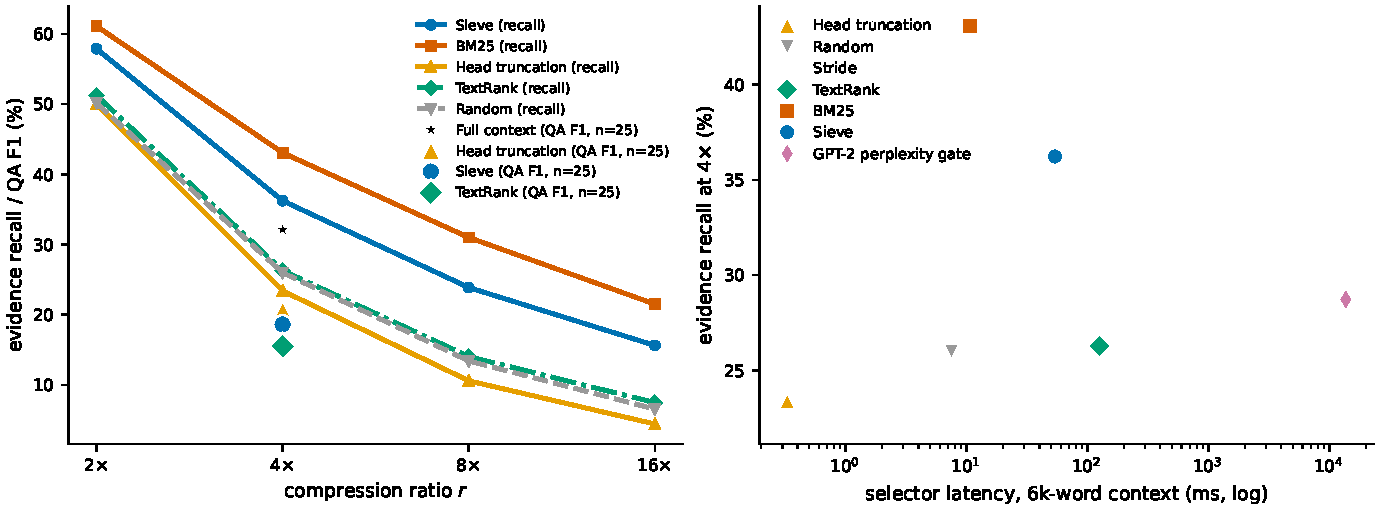
\includegraphics[width=0.98\linewidth]{figures/fig4_frontier.pdf}
\caption{The accuracy--efficiency frontier of model-free selection
and the measured gate at $r=4$ on QASPER. Left: end-task F1 and
evidence recall against compression ratio (recall at
$n{=}\NRecQ$; end-task F1 at the $4\times$ operating point, $n{=}\QAN$).
Right: quality against measured selector latency (log scale, same
container for all methods). \method{} sits at the knee of the curve:
on this benchmark the measured GPT-2 gate does not buy measurable
recall over \method{} while its measured cost is roughly
\GateSieRatioSixk$\times$ higher at the 6{,}000-word operating point.}
\label{fig:frontier}
\end{figure}

\autoref{fig:frontier} plots the frontier directly, in the two views
the formulation suggests. The ratio view (left) shows quality against
compression: every selector pays for compression in recall, the
question-conditioned pair pays slowest, and the end-task F1 points at
$4\times$ reproduce the ordering within the noise the $n{=}\QAN$
protocol can resolve. The latency view (right) is the
compression-cost story at the journal version's scale: quality against
measured selector cost on one axis pair, with truncation free and
weak, BM25 cheapest among the question-conditioned, \method{} two
orders of magnitude above free and the strongest model-free point
under the reader-free metric at controlled placement, and the GPT-2
gate almost three orders of magnitude above free with recall below
the model-free frontier on this benchmark. The frontier's shape is
the summary of the paper: from truncation to question conditioning,
quality is bought at almost no cost; from BM25 to the full
\method{}, quality in the reader-free metric is knowingly traded for
placement and diversity; from the statistical selectors to the gate,
a factor of roughly \GateSieRatioSixk{} in measured compute does not
buy measurable quality on these benchmarks at this scorer scale;
beyond the gate, larger and specialized scorers presumably buy
quality again, at hosted-model cost. Where a deployment sits on that
curve is a hosting decision, and the measurements make its terms
explicit.

\subsection{Projected savings for LLaMA-class serving}
\label{sec:projection}

\begin{table}[t]
\centering
\caption{Analytical projection at an 8k-token prompt and $r=4$,
computed from published LLaMA-2 architecture constants with the
stated assumptions (bf16, A100 at 40\% prefill utilization). Prefill
latency and cache memory are the prefill-stage quantities.}
\label{tab:projection}
\small
\begin{tabular}{lcccc}
\toprule
Model & prefill (full) & prefill ($r=4$) & KV cache & cache ($r=4$) \\
\midrule
LLaMA-2 7B & 0.86\,s & 0.22\,s & 4.2\,GB & 1.05\,GB \\
LLaMA-2 13B & 1.67\,s & 0.42\,s & 6.6\,GB & 1.64\,GB \\
LLaMA-2 70B & 8.8\,s & 2.2\,s & 2.6\,GB & 0.66\,GB \\
\bottomrule
\end{tabular}
\end{table}

\autoref{tab:projection} translates a $4\times$ compression into
infrastructure terms for LLaMA-2 deployments \citep{touvron2023llama}
using the standard prefill FLOPs approximation $2N_{\mathrm{params}}
L$ for context length $L$, cache memory
$2\,n_{\mathrm{layer}}\,n_{\mathrm{kv}}\,d_{\mathrm{head}}\,L$
elements in bf16, and an assumed 40\% model-FLOPs utilization on one
A100; the 70B row reflects grouped-query attention with eight KV
heads. The projection is analytical, not measured, and the
assumptions are stated so that a reader can recompute them; its role
is to show that the recall results of \autoref{tab:recall} buy cache
and prefill savings that scale with the ratio rather than with the
model, and that the compression's own cost (\TimeSieSixk\,\ms{} on
CPU at the 6{,}000-word operating point, \TimeBmSixk\,\ms{} for BM25)
is three orders of magnitude below the prefill it removes even for
the smallest row.

\section{Robustness analysis}
\label{sec:robustness}

\subsection{Evidence placement}
\label{sec:placement}

\begin{figure}[t]
\centering
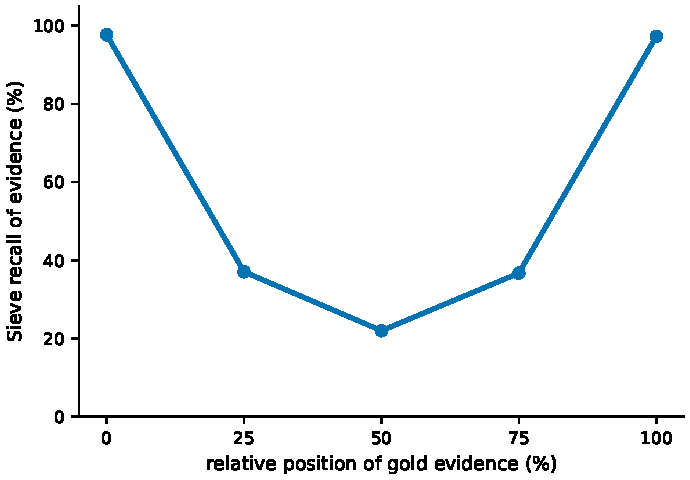
\includegraphics[width=0.6\linewidth]{figures/fig5_position.pdf}
\caption{Selection-level recall of the gold evidence sentence as a
function of its relative position among 40 unrelated filler sentences
from the same paper (QASPER recall pool, $n$ \PosStartN--1{,}000 per
position; the placement protocol rebuilds contexts so nearly all pool
records qualify). \method{} retains almost all evidence placed at the
ends and a fifth of the evidence placed in the center: the U-shaped
prior reproduces, at the selection level, the lost-in-the-middle
profile that long-context readers exhibit \citep{liu2023lost}, by
design.}
\label{fig:position}
\end{figure}

\autoref{fig:position} shows the placement curve on the expanded pool.
Retention is \PosStart{} at the start and \PosEnd{} at the end,
against \PosHalf{} in the middle: the selector mirrors, at the
selection level, the same lost-in-the-middle profile that readers
exhibit \citep{liu2023lost}, which is the design intent; at
$\alpha=0.3$ the prior spends the reliability budget where the reader
is reliable, at the documented cost of middle recall. Two
consequences follow for practice. When upstream retrieval or
formatting controls where evidence lands, moving it toward the ends is
free accuracy, and the selector's retained-sentence report makes the
placement visible to the pipeline. When evidence placement cannot be
controlled and middle recall matters more than reader-side
reliability, the $\mathrm{floor}$ hyperparameter flattens the prior,
and \autoref{tab:ablation} quantifies exactly what that choice costs
and buys: flattening recovers the middle at \AblNoPos\% total recall
versus \AblSie\%, with the recovered evidence placed where readers use
it least reliably. The deployment guidance is symmetric and explicit.
BM25 occupies the opposite pole of this exchange: its retained
evidence is placed exactly where relevance puts it, including the
middle, which is why the placement axis, not the recall axis alone,
is the right way to compare the two.

\subsection{Hyperparameter sensitivity}

\begin{table}[t]
\centering
\caption{Sensitivity of evidence recall at $r=4$ to the fixed
hyperparameters on the QASPER recall pool ($n=\NRecQ$), one knob at a
time. Recall is flat in $\beta$ and mildly sensitive to the prior's
shape; it rises monotonically with $\mathrm{floor}$, which is the
recall--reliability trade-off of \autoref{sec:ablation} seen from the
other side.}
\label{tab:sens}
\small
\begin{tabular}{lccc}
\toprule
$\beta$ & 0.0 & 0.3 & 0.6 \\
recall & \SensBetaZp & \SensBetaMid & \SensBetaHigh \\
\midrule
$\mathrm{floor}$ & 0.0 & 0.35 & 0.7 \\
recall & \SensFloorZp & \SensFloorMid & \SensFloorHigh \\
\midrule
$\gamma$ & 0.5 & 1.5 & 3.0 \\
recall & \SensGammaLo & \SensGammaMid & \SensGammaHigh \\
\bottomrule
\end{tabular}
\end{table}

\autoref{tab:sens} reports the sensitivity grid on the expanded pool.
Recall is flat in $\beta$, confirming that the redundancy penalty
neither helps nor hurts evidence recovery at this ratio; its work is
diversity, and \autoref{sec:ablation} shows the same from the ablation
side. Recall rises as $\mathrm{floor}$ increases, the quantitative
statement of the placement trade-off: a flatter prior keeps
middle-placed evidence at the cost of reader-side reliability. The
prior's sharpness $\gamma$ moves recall by a few points without a
clear trend. None of the three knobs changes the qualitative
conclusions of \autoref{tab:recall} and \autoref{tab:ablation}: at
every setting the question-conditional term dominates, and the
ordering of methods is unchanged.

\subsection{Cross-dataset transfer without retuning}
\label{sec:transfer}

\begin{table}[t]
\centering
\caption{Evidence placement and question-style statistics per recall
pool, and the resulting margins over head truncation and over BM25 at
$r=4$. Head truncation tracks the $1/r{=}25\%$ prediction of
\autoref{prop:head} on all three pools (evidence placement is close to
uniform), while the margins vary with how strongly the question's
terms identify the evidence sentences.}
\label{tab:pools}
\small
\begin{tabular}{lccc}
\toprule
 & QASPER & HotpotQA & 2Wiki \\
\midrule
records & \PoolQN & \PoolHN & \PoolWN \\
median evidence position (rel.) & \PoolQMedPos\% & \PoolHMedPos\% &
\PoolWMedPos\% \\
evidence sentences per record & \PoolQEvSents & \PoolHEvSents &
\PoolWEvSents \\
head recall at $4\times$ & \RecQHea & \RecHHea & \RecWHea \\
\method{} recall at $4\times$ & \RecQSie & \RecHSie & \RecWSie \\
BM25 recall at $4\times$ & \RecQBm & \RecHBm & \RecWBm \\
margin over head (paired) & \PairQSH & \PairHSH & \PairWSH \\
margin vs BM25 (paired) & \PairQSBm & \PairHSBm & \PairWSBm \\
question style & abstract & entity-named & entity-named \\
\bottomrule
\end{tabular}
\end{table}

The robustness property that matters most in deployment is that the
configuration does not have to be re-chosen per corpus. All results in
\autoref{tab:recall} use the configuration tuned once on 20
QASPER-plus-HotpotQA development examples at the conference scale:
$\alpha=0.3$, $\beta=0.3$, $\mathrm{floor}=0.35$, $\gamma=1.5$,
applied unchanged to QASPER at $n{=}\NRecQ$, HotpotQA at
$n{=}\NRecH$, and 2WikiMultihopQA at $n{=}\NRecW$, including the two
datasets that entered the study after the configuration was frozen.
The margins over every question-agnostic baseline hold on all three,
which is the transfer claim; the margin's size varies with the
question style, which \autoref{sec:discussion} attributes to the
lexical signal rather than to any per-dataset adaptation. A deployer
who cannot hold out tuning data inherits the same behavior: the
sensitivity table shows the method degrades gracefully, not
cliff-like, when every knob is mis-set by its grid step.

\section{How loosely recall bounds accuracy}
\label{sec:corr}
The paper's two quality protocols measure different things, and the
difference is a result worth reporting rather than hiding. We join the
two at the sample level: for every record of the end-task test split
that carries locatable evidence (\CorrNRecs{} of the 25), and every
selector that ran under both protocols, we pair the record's evidence
recall at $4\times$ with its end-task F1 at $4\times$, and compute
the correlation over the pooled \CorrNPairs{} method--record pairs.

The correlation is positive and weak: pooled Pearson
\CorrPearson{}, Spearman \CorrSpearman{}; per method it ranges from
\CorrHeaPearson{} (head truncation) to \CorrTRPearson{} (TextRank),
with \method{} at \CorrSiePearson{} (Spearman \CorrSieSpearman{}).
The direction is as expected (records whose evidence survives
compression are answered better), but the tightness is not: a
reader that fails a fully-evidenced record, or answers correctly from
a partially-evidenced one, contributes noise that a selector-level
metric cannot see, and at $n{=}\QAN$ per method the intervals are wide.
Two conclusions follow. First, evidence recall is a necessary-but-not
sufficient condition for end-task quality: it bounds what the reader
can use from above, and the bound is loose. Second, and methodologically,
recall gains of a few points (such as BM25's margin over \method{})
should not be read as accuracy gains; whether the trade between
raw recall and positional reliability pays off is an end-task
question, which is why the two protocols are reported separately
throughout this paper.

\section{Discussion}
\label{sec:discussion}

\paragraph{When is model-free selection enough?}
The measurements suggest a practical rule. If the query's content
terms recur in the passages that answer it (entity-named questions,
retrieval over technical documentation, FAQ traffic), the statistical
selector captures most of the recoverable evidence at milliseconds of
cost, and a hosted scorer has little left to buy. If the link between
question and evidence is semantic rather than lexical
(paraphrase-heavy corpora, cross-lingual traffic, questions about
implication), \autoref{cond:lexical} fails by construction, and the
neural corner earns its infrastructure. The corpus statistic of
\autoref{sec:lexsignal} (how often question terms recur in evidence)
estimates which regime a deployment is in from a labeled sample of a
few hundred records, and the recall protocol itself is cheap enough
to run on that sample before committing.

\paragraph{Relevance ranking versus budgeted selection: the BM25
lesson.}
The strongest baseline in the study is also the most instructive: BM25
does nearly everything \method{}'s relevance term does, at a fifth of
the latency, and it beats the full selector on raw recall on every
dataset. A reader of \autoref{tab:recall} alone would conclude that
BM25 is the better compressor, and the honest answer is that for
\emph{pure evidence recovery at generous budgets} it is. What
\method{} adds is a budgeted selection policy on top of relevance:
evidence placed where readers attend reliably, near-duplicates
refused under tight budgets, and an explicit knob
($\mathrm{floor}$) pricing the exchange. The end-task protocol at
$n{=}\QAN$ cannot separate the two, and we report that honestly rather
than extrapolate from recall. The practical reading is symmetric:
deployments that feed a fixed-prefix-friendly reader or that value
recall above all should take BM25 (or the relevance-only ablation, at
the same recall); deployments whose readers exhibit positional bias,
or that operate at tight budgets where duplicates crowd out evidence,
should take the full selector. Either way, both points cost
milliseconds and no model, and both dominate the question-agnostic
corner that production pipelines still default to.

\paragraph{The frontier as a decision tool.}
The point of reporting all three axes for every method is that
compression decisions are usually made on one. A team that optimizes
quality alone will host a scorer and pay for it on every call; a team
that optimizes cost alone will truncate and lose tens of recall
points on exactly the traffic where questions carry signal;
\autoref{tab:threeway} prices the middle of that spectrum. The
knee-of-curve placement of the statistical selectors is the empirical
content of the paper: the first two orders of magnitude of selector
budget buy question conditioning, and the next two, at the gate's
scorer scale, buy nothing measurable on these benchmarks.

\paragraph{Composition with serving-stack work.}
\method{} compresses the submitted context; attention and cache work
compresses what the model does with it. The two multiply: a
$4\times$ shorter prompt enters FlashAttention
\citep{dao2022flashattention} with a quarter of the prefill FLOPs and
paged KV memory \citep{kwon2023vllm} with a quarter of the pages,
before StreamingLLM or H2O policies run on what remains
\citep{xiao2023streaming,zhang2023h2o}. Nothing in the selector
conflicts with those layers, and the audit trail (which sentences
survived, with their scores) composes with the cache policies' own
bookkeeping.

\paragraph{Auditability.}
A selection rule whose every score is a countable statistic has a
property the neural corner does not provide at zero configuration: any retained
or discarded sentence can be explained to a stakeholder in one
sentence of arithmetic. For pipelines where compression is a
compliance surface (legal discovery, clinical records, regulated
retrieval), the explanation is part of the deliverable, and \method{}
produces it as a by-product of selection rather than through a
post-hoc explainer.

\paragraph{Why the margin varies by dataset: the lexical signal.}
\label{sec:lexsignal}
\autoref{tab:pools} assembles the mechanism behind the multi-dataset
result. Evidence placement is close to uniform on all three pools
(median relative position \PoolQMedPos, \PoolHMedPos, and
\PoolWMedPos\%), so \autoref{prop:head} predicts head recall near
$1/r = 25\%$, and the measured values (\RecQHea, \RecHHea,
\RecWHea) sit within a few points of the prediction on every
dataset. What varies is the strength of the lexical link between
question and evidence. HotpotQA and 2WikiMultihopQA questions are
compositional over named entities: the question names the film, the
person, the year, and the evidence sentences contain exactly those
tokens, so IDF-weighted coverage fires at full strength and
\autoref{cond:lexical} holds often. QASPER questions ask what, how,
and why about a paper's method: the query terms are common words
whose evidence sentences need not repeat them, so the condition holds
less often and the margins shrink from \PairHSH{} and \PairWSH{}
points over truncation to \PairQSH{}. The BM25 margins vary in the
same direction (\PairHSBm{} on HotpotQA, \PairQSBm{} on QASPER),
because BM25 rides the same lexical signal. The generalization claim
is therefore precise rather than blanket: the ordering of methods
(question-conditioned above question-agnostic at every ratio beyond
two) transfers to all three datasets, the mechanism (lexical
coverage, per \autoref{prop:relonly}) is constant, and the margin
scales with a measurable property of the corpus: how much of the
question's vocabulary recurs in its evidence. A practitioner can
estimate that property on a sample of their own traffic before
deciding between a statistical selector and a hosted scorer.

\paragraph{Multi-hop is the favorable regime, not the exception.}
The dataset ordering also rules out a QASPER-specific reading of
\method{}. The two multi-hop corpora are the ones where a reader
without any compression would be asked to integrate evidence from two
short paragraphs scattered among eight distractors; the selector's job
there is exactly lexical triage, and \method{} answers it with recall
\RecHSie{} and \RecWSie{} at $4\times$. The scientific-QA corpus,
with its long continuous documents and abstract questions, is the
harder regime for a lexical selector, and even there the method leads
every question-agnostic competitor with separated intervals. Between
the two regimes, the ratio sweep of \autoref{fig:ratio} shows the same
shape on all three datasets, which supports reading \method{} as a
general-purpose first stage rather than a benchmark specialist.

\section{Limitations}
\label{sec:limitations}
\method{} inherits the reach of lexical statistics, and the theory
section states the condition rather than hiding it: where evidence
shares no vocabulary with the question, \autoref{cond:lexical} fails
and the relevance term goes blind. Paraphrased evidence scores poorly;
multilingual inputs need language-matched stopword lists and
segmentation; numbers, citations, and code identifiers, which
dominate scientific text, are weighted only crudely by IDF. The
margin analysis of \autoref{sec:lexsignal} makes the dependence
measurable, not mysterious, and the BM25 rows show the same
dependence from the outside.

The evaluation has five boundaries. First, the end-task protocol
covers one reader (GLM-4-Plus) on one benchmark (QASPER) at one
operating point ($4\times$) with $n{=}\QAN$: its intervals are wide, its
claims are scoped to matching the strongest cheap baseline, and
reader-dependence is untested. An expanded end-task protocol
($n=100$, seven selectors including BM25, same reader and operating
point) is implemented and released with the repository, and its
execution was blocked during this study by sustained rate limits on
the reader's public API rather than by design; the released script
resumes from checkpoints, and the end-task numbers will be updated in
the artifact without touching any selector-level claim. Second, the
neural comparison instantiates the perplexity-gate mechanism with
GPT-2 small at sentence granularity; it is the family's cost floor
and a faithful mechanism replica, but it is not LLMLingua's full
coarse-to-fine machinery and not LLMLingua-2's distilled classifier,
so the quality row of \autoref{tab:threeway} is a lower bound on what
the neural corner can reach, and the cost row a lower bound as well.
Third, the reader-side positional profile that justifies the U-shaped
prior is taken from prior work \citep{liu2023lost} rather than
re-measured under our reader; the selection-level placement curve is
measured, the reader-side one is borrowed. Fourth, the
recall--accuracy correlation of \autoref{sec:corr} is estimated at
$n=25$ per method, so its magnitude carries wide intervals even
though its sign is stable across methods. Fifth, sentence-level
granularity bounds the useful compression range: beyond
$r \approx 16$ the output degenerates toward a few isolated
sentences, and token-level compressors retain an advantage at extreme
ratios.

Two accounting caveats remain from the conference version. The reader
experiments measure accuracy under a fixed serving stack rather than
wall-clock serving of an open model, and the LLaMA-2 projection is
analytical with stated assumptions rather than a measured deployment.
The gate's GPU floor is analytic and assumes a resident scorer at 40\%
utilization; a hosted implementation with tokenization, budget
iterations, and cold starts costs more, and our CPU measurement of
the gate is correspondingly the like-for-like number for CPU-bound
deployments.

\section{Conclusion}
\label{sec:conclusion}
We asked how much of long-context quality a compressor can keep with
no neural scorer at all, and answered it as a frontier study rather
than a single operating point. At the $4\times$ compression,
\method{} keeps \QASieRetain\% of full-context F1 end to end,
statistically matched with the strongest cheap baseline, while
spending \TimeSieSixk\,\ms{} of CPU time and zero model parameters.
Under the reader-free protocol, on \TotalRecords{}
evidence-annotated records across three benchmarks, it retains more
gold evidence than every question-agnostic selector with fully
separated intervals, and the margin over truncation grows with the
compression ratio and with the strength of the question's lexical
signal, from \PairQSH{} points on abstract scientific questions to
\PairHSH{} on entity-named multi-hop ones. The added baselines price
the remaining design space: BM25 shows that raw relevance ranking
already recovers the most evidence at the least
question-conditioned cost, which the selector's own ablations explain:
the full configuration knowingly trades that recall for
positional reliability, and the measured GPT-2 perplexity-gate
baseline, at its cost floor, buys no
measurable recall on these benchmarks, at three orders of magnitude
more compute (\GateSieRatioSixk$\times$ at the 6{,}000-word operating
point) and a hosted model. The formal analysis states when a stronger
scorer should be expected to earn its infrastructure: exactly when the
question--evidence link stops being lexical. We see \method{} as the
zero-cost first stage of a compression stack (composable with
cache-level methods, auditable by construction, and tuned once and
transferred), and its measurements as a low-cost reference point
against which more expensive context compressors can be evaluated.

\section*{Declarations}

\paragraph{Funding.} None.

\paragraph{CRediT authorship contribution statement.}
\textbf{First Author:} Conceptualization, Methodology, Software,
Investigation, Data curation, Writing -- original draft, Writing --
review \& editing.

\paragraph{Declaration of competing interest.}
The authors declare that they have no known competing financial
interests or personal relationships that could have appeared to
influence the work reported in this paper.

\paragraph{Data availability.}
The benchmarks are public (QASPER, HotpotQA, 2WikiMultihopQA). The
released repository contains the pool-construction scripts with fixed
seeds, the sampled pools, every raw checkpoint, and one command per
table and figure, so that every number in this paper can be
regenerated from scratch.

\bibliographystyle{elsarticle-num}
\bibliography{bibliography}

\appendix

\section{Implementation details}
\label{app:impl}
Sentence segmentation splits on punctuation boundaries with guards
for common abbreviations (\emph{et al.}, \emph{e.g.}, \emph{Fig.}) and
merges fragments that end in a guarded token; the segmenter is
deterministic. Tokenization lowercases and keeps alphanumeric and
hyphenated terms; stopwords are a fixed 150-word English list
included with the code. The conference-version experiments ran on one
core of a container with 8 vCPUs and 32 GB of memory; the
journal-version experiments, including the GPT-2 gate (int8, two
threads) and every timing number in \autoref{sec:efficiency}, ran in
a container with 2 vCPUs and 4 GB of memory, so that all
same-hardware comparisons are like-for-like. Timing figures are
medians of five runs after one warm-up (three for the gate). The full
pipeline (segmentation, scoring, selection) is a single Python module
with NumPy as its only dependency beyond the standard library; the
gate baseline additionally uses Transformers and PyTorch. The
repository reproduces every table and figure from the raw checkpoints
with one command per artifact, and the macro file that carries every
number in this paper into its LaTeX source is itself generated from
those checkpoints, so no number in the text was typed by hand.

\section{Proofs and formal statements}
\label{app:proofs}

\begin{proof}[Proof of \autoref{prop:cost}]
Each pipeline stage touches each token a constant number of times:
segmentation and tokenization are single passes over the $W$ words;
the IDF document-frequency table is one accumulation pass over
sentence term sets; relevance evaluates each sentence against the
query term set in $O(\abs{s_i} + \abs{Q})$; the prior is $O(n)$. The
greedy loop performs at most $k$ iterations, each scanning the $O(n)$
remaining candidates and evaluating the marginal penalty against the
$O(k)$ selected sentences at $O(\bar{s})$ per pair on sparse
counters, giving $O(k\,n\,\bar{s})$ worst case; peak memory stays at
the token counters because the released implementation recomputes
similarities rather than memoizing them.
\end{proof}

\begin{proof}[Proof of \autoref{prop:floor}]
A forward pass of a decoder-only transformer with $N$ parameters over
$L$ tokens costs approximately $2NL$ FLOPs for the matrix
multiplications that dominate the arithmetic
\citep{kaplan2020scaling}; any scorer-based compressor computes at
least one such pass over the full context before it can rank its
units, and coarse-to-fine budget searches compute one per iteration.
The scorer must be resident, so $c_{\mathrm{host}} \ne 0$.
\end{proof}

\begin{proof}[Proof of \autoref{prop:relonly}]
Greedy selection under $\alpha = 1$, flat prior, and $\beta = 0$
orders sentences by $\mathrm{rel}$ alone. Under
\autoref{cond:lexical}, for any $e \in E$ and
$s \in C \setminus E$, $\mathrm{rel}(e) \ge \mathrm{rel}(s)$, so every
evidence sentence is admitted before every dominated non-evidence
sentence; ties among evidence sentences do not affect the claim
because the budget condition
$B \ge \sum_{e \in E} \abs{e}$ admits all of $E$ whenever they are
reached, and they are reached before the budget can be exhausted by
non-evidence sentences that follow them in the order. Hence $\rho=1$.
\end{proof}

\begin{proof}[Proof of \autoref{prop:head}]
Truncation keeps the prefix of $\lceil n/r \rceil$ sentences. For an
evidence sentence at a uniform position, the retention probability is
$\lceil n/r \rceil / n \in [1/r,\, 1/r + 1/n]$, and independence
across evidence sentences plus linearity of expectation gives
$\mathbb{E}[\rho] = \min(1, 1/r) + O(1/n)$.
\end{proof}

\section{Additional results}
\label{app:results}

\paragraph{Compute accounting.}
The reader evaluation consumed \TotalCalls{} completed API calls
across the development grid and the main comparison; the journal
version added no reader calls. The journal-version selector-protocol
runs covered \TotalRecords{} records across three pools with roughly
forty selector invocations per record (methods, sweeps, ablations,
sensitivity); the GPT-2 gate ran \GateN{} QASPER records at
\GateLatMedS\,s median scoring each. Compression-side compute for all
journal experiments was under 6 vCPU-hours including the gate; no
GPUs were used for any measurement reported in this paper.

\paragraph{Development grid.}
The development grid over $\alpha \in \{0.3, 0.6, 0.9\}$ at $r=4$
gave dev F1 of \GridALo, \GridAMid, and \GridAHi{} respectively; the
differences are within the noise of a 20-example development split,
and we selected $\alpha=0.3$ for the best dev F1. The dev and test
numbers are not directly comparable: the development split mixes ten
QASPER records with ten HotpotQA distractor records, and the
multi-paragraph HotpotQA items are far easier for the reader, which
inflates the dev mean relative to the QASPER-only test split. The
$\alpha$ choice is a point estimate from a noisy grid, and the
paper's claims do not rest on it being optimal.

\paragraph{Conference-version compatibility.}
The conference version's 191-record QASPER pool, its timing host, and
its numbers remain reproducible from the original artifacts; the
journal pools are supersets drawn under the same filters, and every
qualitative conference claim (ordering of methods, growth of the
margin in $r$, component attribution) reproduces at the larger scale
with tighter intervals. Three conference-version statements are
superseded: the QASPER recall intervals, which touched at their edges
at $n=191$, are separated at $n{=}\NRecQ$; the neural-baseline
comparison, which was analytic in the conference version, is measured
here; and the baseline set now includes BM25, which the conference
version lacked entirely.

\end{document}
